%%%%%
%%
%% Sample document ``thesis.tex''
%%
%% Version: v0.2
%% Authors: Jean Martina, Rok Strnisa, Matej Urbas
%% Date: 30/07/2008
%%
%% Copyright (c) 2008-2011, Rok Strniša, Jean Martina, Matej Urbas
%% License: Simplified BSD License
%% License file: ./License
%% Original License URL: http://www.freebsd.org/copyright/freebsd-license.html
%%%%%

% Available documentclass options:
%
%   <all `report` document class options, e.g.: `a5paper`>
%   withindex   - enables the index. New index entries can be added through `\index{our entry}`
%   glossary    - enables the glossary.
%   techreport  - typesets the thesis in the technical report format.
%   firstyr     - formats the document as a first-year report.
%   times       - uses the `Times` font.
%   backrefs    - add back references in the Bibliography section
%
% For more info see `README.md`
% \documentclass[times]{cam-thesis}
\documentclass[a4paper,12pt,twoside,openright]{article}

% Citations using numbers
% \usepackage[numbers]{natbib}

\usepackage[style=authoryear]{biblatex} %Imports biblatex package
\addbibresource{icassp.bib,bibliography.bib}
% \addbibresource{icassp.bib}

\usepackage{xcolor}
\usepackage{caption}
\usepackage{subcaption}
\usepackage{amsmath}
\usepackage{amssymb}
\usepackage{sectsty}
\usepackage{booktabs}
\usepackage{hyperref}
\usepackage{caption}
\usepackage{subcaption}
\usepackage{graphicx}
\usepackage{upgreek}
\usepackage{dsfont}
\usepackage{bbm}

% \usepackage[T1]{fontenc}
% \usepackage{crimson}
% \usepackage{fbb}
% \usepackage{charter}
% \usepackage{imfellEnglish}
% \usepackage{euscript}
\usepackage{biolinum}
% \usepackage{helvet}
% \usepackage{tgpagella}
% \usepackage{fbb}
\usepackage{tgpagella}
% \usepackage{times}

% \usepackage{libertine}
% \usepackage{libertinust1math}

% \renewcommand{\sfdefault}{ppl}

%\setlength{\parindent}{0em}
%\setlength{\parskip}{1em}

\newcommand{\crit}[1]{\textcolor{red}{#1}}
\newcommand{\draft}[1]{\textcolor{blue}{#1}}
\newcommand{\ind}{\perp\!\!\!\!\perp} 
\newcommand{\fzero}{F\textsubscript{0}}

%%%%%%%%%%%%%%%%%%%%%%%%%%%%%%%%%%%%%%%%%%%%%%%%%%%%%%%%%%%%%%%%%%%%%%%%%%%%%%%%
%% Thesis meta-information
%%

%% The title of the thesis:
\title{\bf Groups of high-dimensional data}

%% The full name of the author (e.g.: James Smith):
\author{Dan Andrei Iliescu}

%% College affiliation:
% \college{St Edmund's College}

%% College shield [optional]:
% \collegeshield{CollegeShields/Christs}
% \collegeshield{CollegeShields/Churchill}
% \collegeshield{CollegeShields/Clare}
% \collegeshield{CollegeShields/ClareHall}
% \collegeshield{CollegeShields/CorpusChristi}
% \collegeshield{CollegeShields/Darwin}
% \collegeshield{CollegeShields/Downing}
% \collegeshield{CollegeShields/Emmanuel}
% \collegeshield{CollegeShields/Fitzwilliam}
% \collegeshield{CollegeShields/Girton}
% \collegeshield{CollegeShields/GonCaius}
% \collegeshield{CollegeShields/Homerton}
% \collegeshield{CollegeShields/HughesHall}
% \collegeshield{CollegeShields/Jesus}
% \collegeshield{CollegeShields/Kings}
% \collegeshield{CollegeShields/LucyCavendish}
% \collegeshield{CollegeShields/Magdalene}
% \collegeshield{CollegeShields/MurrayEdwards}
% \collegeshield{CollegeShields/Newnham}
% \collegeshield{CollegeShields/Pembroke}
% \collegeshield{CollegeShields/Peterhouse}
% \collegeshield{CollegeShields/Queens}
% \collegeshield{CollegeShields/Robinson}
% \collegeshield{CollegeShields/Selwyn}
% \collegeshield{CollegeShields/SidneySussex}
% \collegeshield{CollegeShields/StCatharines}
% \collegeshield{CollegeShields/StEdmunds}
% \collegeshield{CollegeShields/StJohns}
% \collegeshield{CollegeShields/Trinity}
% \collegeshield{CollegeShields/TrinityHall}
% \collegeshield{CollegeShields/Wolfson}
% \collegeshield{CollegeShields/FitzwilliamRed}

%% Submission date [optional]:
% \submissiondate{June, 2023}

%% You can redefine the submission notice [optional]:
% \submissionnotice{A badass thesis submitted on time for the Degree of PhD}

%% Declaration date:
\date{20 Oct 2023}
\title{Chapter 3: Imputation on unseen patterns of missingness}

%% PDF meta-info:
% \subjectline{Computer Science}
% \keywords{one two three}

\newcommand{\flag}[1]{\textcolor[rgb]{0.9,0.3,0.3}{\textbf{#1}}}


%%%%%%%%%%%%%%%%%%%%%%%%%%%%%%%%%%%%%%%%%%%%%%%%%%%%%%%%%%%%%%%%%%%%%%%%%%%%%%%%
%% Contents:
%%
\begin{document}

\allsectionsfont{\sffamily}

%%%%%%%%%%%%%%%%%%%%%%%%%%%%%%%%%%%%%%%%%%%%%%%%%%%%%%%%%%%%%%%%%%%%%%%%%%%%%%%%
%% Title page, abstract, declaration etc.:
%% -    the title page (is automatically omitted in the technical report mode).
% \frontmatter{}

%%%%%%%%%%%%%%%%%%%%%%%%%%%%%%%%%%%%%%%%%%%%%%%%%%%%%%%%%%%%%%%%%%%%%%%%%%%%%%%%
%% Thesis body:
%%

% \chapter*{Amortised imputation in partial observations}

\maketitle

\tableofcontents

\begin{abstract}
    This chapter explores the application of our latent-group generative model to the problem of missing data imputation (MDI) in the context of high-dimensional data. This is the problem of filling in missing observations within a ``data structure'' \crit{(Be more precise. A data structure is not the whole dataset, but just one element in the dataset.)} --- such as a multivariate time-series, image, or data table --- conditionally on the observations that are available. We are considering patterns of missingness of the missing-not-at-random (MNAR) type, meaning that whether or not an observation is missing might depend on the value of any variable, including the outcome. Take this as an example.
\end{abstract}

\section{Introduction}

\crit{Damon: New plan for chapter on missing data imputation: 1. First start with the setup. Don't mention group-based inference. 1.a. Introduction: missing values, quick intro to prosody control, why this is worth doing. 1.b. Abstract formulation. 1.c. Concrete example: audio. 1.d. Another example: images. 2. Then discuss my proposed solution.}

\subsection{Territory}

\draft{We want to train a model on complete data that can impute missing features at test time across a range of different patterns of missingness.}

There are many real-world problems of this form, including time-series forecasting, image inpainting, matrix completion, etc.

We are looking at problems with inferring the complete datapoint from partial observations.

We have complete data during training and missing data during testing. We want to fill in the missing data.

You have learned a joint distribution over the dimensions of a variable $Y$. You are given a set a dimensions (called the context set) $Y_C$ and you want to estimate the probability of the rest of the dimensions (the target set) $P(Y_T | Y_C)$. The standard approach is to train the model by sampling a selection variable $M$ assigning each dimension of $Y$ to either the context set or the target set.

1. Practically, it's common knowledge that the split between context and target affects what you end up learning. 1. In computer vision, everyone knows that you can't train a model with Bernoulli random missingness and expect it to correctly impaint a large contiguous region of the image. 2. In time-series forecasting / language modelling, it's a common approach to vary the length of the context set, because it produces more robust results than simply forecasting. Also, we all know that a model trained to predict the next time-step will explode when asked to predict the next 100 timesteps. 3. Also, what is the difference between language modelling and text embeddings? The pattern of missingness during training.

We don't quite understand why the distribution that we choose for $M$ affects the learned distribution $P(Y_T | Y_C)$. 

2. But there is not theoretical framework for understanding what's going on here. The theory of missing data imputation deals with situations where you don't see the complete data, but you see the missingness pattern that you will encounter during testing. This situation is the opposite: You can perfectly model the data, but you don't know what the missingness pattern will be during testing.
    1. Theoretically, if you can learn the joint distribution of the data, you also get the conditional distribution for free. Let's look at an example. Usually, generative models map a latent variable $Z$ to an observed variable $Y$. If we assume that the generative model is correct, than we can infer $Z$ from the partial observation using expectation maximisation, whatever the pattern of missingness is.
    2. However, this method is slow. In practice, we want to do amortised inference. We want to learn a model $\phi$ to sample the latent variable. 
    3. And here is the problem. Even if $\theta$ might be the correct generative parameter, $\phi$ might be wrong.

Neural processes are the answer to How do I fill in missing data with group-aware modelling?. But if you pitch this chapter as Naive group-based models turn out not to work well for extrapolation, and I claim the answer lies in having an explicit model of missingness. You are positioning yourself as an accompaniment to anyone who wants to learn functions using neural networks.

Existing methods have difficulty solving this problem because 1) they do not generalise well to unseen patterns of missingness, and 2) they use the available data inefficiently.

\subsection{Niche}

\draft{Why is it that when we train an imputation model with simulated 0.5 Bernoulli missingness, the imputation model does not generalise well to different patterns of missingness, even though the distribution of missingness theoretically puts non-zero probability on every possible pattern of missingness.}

2. **Niche.** How can we train for an unknown pattern of missingness (or possibly multiple patterns)?
   1. **Context.** What is in the territory but isn't in the niche? Training for specific patterns of missingness, like forecasting, superresolution, inpainting, interpolation, extrapolation.
   2. **Problem.** Even though many streams of research have independently identified that training with different patterns of missingness has an impact over how well the model generalises, we don't have an overarching explanation for why this happens.
   3. **Example.** How can I illustrate the problem? I can train the same image model with different patterns of missingness and then test it on every possible pattern of missingness. 
      1. I can plot the reconstruction loss as a function of certain statistics about the missingness pattern, like the number of missing features, or the entropy of the typicality of the pattern.
      2. I can rank missingness patterns in terms of reconstruction loss for a few different images in the dataset.
   4. **Impact.** Achieving robust imputation can unlock problems where the true pattern of missingness is unknown.

There seems to be a problem with inferring the missing features, but no one has described it coherently.
   1. What are some examples? Varying the size of the context set helps with generalisability. 
   2. Is this the same as missing data imputation? No.
   3. A very important point is that we could train the missingness through expectation maximisation and achieve an unbiased estimator.

   \paragraph{Missing-not-at-random.} We can't just use any method for imputation here, because the data is MNAR. This means that whether or not the data is missing depends on the value of the acoustic features themselves. For example, if the user decides to only provide values for the stressed word in the sentence (and this is a realistic use case), then the provided values will, on average, have higher pitch than the rest of the sentence. Normal imputation methods using deep learning, like Denoising VAE, GAN, Diffusion models, Transformers, don't impute well in this situation. Neither do Gaussian Processes or Neural Processes.

\paragraph{Why is this important?} Missing-not-at-random is a very common situation. One situation is self-censoring. Another is the shared parameter model.

\paragraph{Why do existing models not work in this situation?} Existing models don't work in our situation because our situation is very specific. Usually, people assume that the training setup is identical to the testing data: namely we have the same pattern of missingness. What they do is train a full generative model and then infer the missing data as a latent variable. But this is not our setting. In our setting, we don't know exactly what the patterns of missingness will be at test time. However, during training we have as much complete data as we want. 

\section{Problem statement}

\draft{In its purest form, the problem involves 4 random variables and two parameters: $Y_d$ is the value of the $d$-th dimension of the full observation. $Y_d$ is generated }

\draft{The setup is that during training we have i.i.d. samples of full observations. During testing, however, we can only see the partial observations. The partial observations are generated by combining the full observations (still i.i.d.) with a selection mask. The distribution of the selection mask is unknown, but we assume it's independent of the observation. We want a model that can fill in the missing dimensions of the partial observations as well as possible across the unkown masking distribution during testing. We may be able to make some assumptions about the missingness pattern depending on the real problem that we are addressing, so even though we are looking for a general solution to this problem, we want this general solution to accommodate specific knowledge we might have about the missingness pattern.}

\section{Background}

\crit{[WIP] Damon: Present off-the-shelf solutions in a neutral manner, as their authors intended them.}

% \crit{[TL;DR] Existing methods for missing-data imputation are not sample efficient and they are not robust to changing patterns of misssingness. [WIP] Skip reading the literature review section. It has all the content but it's not fleshed out yet.}

% \paragraph{These are the current solutions to this problem} \crit{What are the traditional solutions to deal with missing data imputation?}

% \paragraph{This is where they go wrong} \crit{The traditional methods are not expressive enough. The zero imputation methods suffer from sparsity }

% \paragraph{Broader context. This is what we're not considering and this is why.} \crit{Related but distinct problems. We are not doing matrix completion. We are not (only) doing time-series forecasting. We are not (only) doing image superresolution and imputation. We are not doing prediction with missing values. We are not doing single function approximation. We are not doing missing not at random. We are not doing unconditional time-series or image models.}

% \begin{itemize}
%     \item Improving the imputation technique for missing values is not always useful for prediction \parencite{lemorvanWhatGoodImputation2021}.
%     \item BERT uses a masked language model training objective. This is equivalent to doing missing value imputation during training with 15\% of the tokens missing completely at random \parencite{devlinBERTPretrainingDeep2019}.
%     \item The basic approach for dealing with missing values in with VAEs is to fill missing values with a default value (say 0) and measuring the reconstruction error on the available values \parencite{nazabalHandlingIncompleteHeterogeneous2020}.
%     \item Another approach is GP-VAE. The samples are autoencoded with convolutions and then a Gaussian Process is trained on the latent representations \parencite{fortuinGPVAEDeepProbabilistic2020}.
%     \item A deep learning framework for predicting climate data \parencite{amatoNovelFrameworkSpatiotemporal2020}.
%     \item A Transformer based method for spatio-temporal data where imputation is based on cross-sectional features \parencite{maCDSACrossDimensionalSelfAttention2019}.
%     \item Multivariate time-series representation learning \parencite{zerveasTransformerbasedFrameworkMultivariate2021}.
%     \item Multivariate time-series imputation with Graph Neural Networks \parencite{ciniFillingApMultivariate2022}. Also found for power-grids \parencite{kuppannagariSpatioTemporalMissingData2021}.
%     \item This review of diffusion models looks at how diffusion models are applied for time-series imputation and image inpainting \parencite{yangDiffusionModelsComprehensive2022}. RePaint is a state-of-the-art image imputation method that, at each stage of the denoising process, replaces the parts of the generated image with a noisy version of the available parts of the ground-truth \parencite{lugmayrRePaintInpaintingUsing2022}. At each denoising stage, it does 10 additional steps of adding noise and then re-sampling in order to preserve coherence. Another approach for time-series imputation is the Conditional Score-based Diffusion Models, where each step of the diffusion model is conditioned on the available data \parencite{tashiroCSDIConditionalScorebased2021}.
%     \item We found a paper using Gaussian Processes as mixed-effects models with a learnable covariance matrix, and they apply it to making predictions about school data \parencite{bonillaMultitaskGaussianProcess}. This is a paper using Gaussian Processes for missing data imputation \parencite{jafrastehGaussianProcessesMissing2022}.
%     \item This paper shows that, even when data is missing completely at random, zero imputation leads to bias in the result increasing with the percentage of missing values \parencite{yiWhyNotUse2019}.
%     \item PartialVAE is close to what I am proposing. A VAE-based method with a PointNet encoder where the value of the element in the set is multiplied with the learned positional embedding. This is used for active learning \parencite{maEDDIEfficientDynamic2019}. For high-dimensional data tabular data (a matrix of examples and features), we have the Partial VAE, a very similar method to ours where the group of data is aggregated by a permutation-invariant function. The datapoints are an elementwise multiplication between the value and the positional embedding. They had the idea of using positional encoding for features that are not spatio-temporal.
%     \item Neural processes are function approximators, probabilistic processes, they are distributions over functions \parencite{garneloConditionalNeuralProcesses2018}. But do they use positional embeddings? They must do something for that covariance function. Positional embeddings are like the covariance function. Anyway, they don't consider the pattern of missingness. In other words, the covariance function should not be independent of the relationship between the context set and the target set. Attentive neural processes aggregate information using a self-attention mechanism \parencite{kimAttentiveNeuralProcesses2019}.
%     \item Structured state spaces seem interesting for modelling sequences \parencite{guEfficientlyModelingLong2022}.
%     \item Multiple-instance learning with attention is a method for getting a fixed-dimensional representation from a set of data, enabling the representation to incorporate structures at multiple levels \parencite{ilseAttentionbasedDeepMultiple2018}. Deep Sets are a more rudimentary method for aggregating data in observations \parencite{zaheerDeepSets2017}.
% \end{itemize}

% \subsection{Vector Autoregressive models}

% Vector Autoregression (VAR) is an econometric model used to understand how an entire system of related variables affects each other. These models generalize the univariate autoregressive model (AR model) by allowing for more than one evolving variable. All variables in a VAR are treated symmetrically; each variable has an equation explaining its evolution based on its lags and the lags of all the other variables.

% A VAR model of order p (VAR(p)) includes p lags of all variables on the right-hand side of each equation. For a k-dimensional time series {Yt}, a VAR(p) model is:

% Yt = A1Yt-1 + A2Yt-2 + ... + ApYt-p + B + Et

% Here, A1, ..., Ap are (k x k) coefficient matrices and B is a (k x 1) vector of constants. The error term Et is a k-dimensional white noise process with time-invariant covariance matrix.

% For missing data imputation, one can utilize the structure of the VAR model. If a value from a variable is missing, we can use the information from other variables and their lags to estimate the missing value. In the context of high-dimensional data, like multivariate time-series or images, this becomes very powerful as it allows leveraging the interdependencies between variables or features to estimate the missing values, which could be more accurate than treating each feature independently.

% \paragraph{Example paper} The principles of VAR models have been widely used in econometrics and other fields with multivariate time-series data. For an example of VAR model usage, Seminal paper by Sims, Christopher A. (1980). "Macroeconomics and Reality". This paper doesn't specifically address missing data imputation but provides a strong foundation for understanding how VAR models can capture and utilize interdependencies between variables in a multivariate time-series context.

% \paragraph{Advantages and Disadvantages} Advantages of the VAR model for missing data imputation:

% \begin{enumerate}
%     \item \textbf{Leverages Interdependencies}: VAR models can capture the relationships between different variables (or features) in a multivariate time-series dataset. This is particularly valuable for high-dimensional data where variables often have complex relationships with each other.
%     \item \textbf{Flexible Lag Structure}: VAR models allow for flexible lag structures, enabling the model to capture temporal dependencies across different time scales.
% \end{enumerate}

% Disadvantages of the VAR model for missing data imputation

% \begin{enumerate}
%     \item \textbf{Parameter Estimation Can Be Challenging}: As the dimensionality of the data increases, the number of parameters in a VAR model grows quadratically, making the model more complex and potentially more challenging to estimate accurately.
%     \item \textbf{Linearity and Stationarity Assumptions}: Similar to the ARIMA model, VAR models assume the data are stationary and the relationships are linear. These assumptions may not hold in all real-world, high-dimensional datasets.
%     \item \textbf{Computationally Intensive}: Due to the large number of parameters and the need to invert large matrices, VAR models can be computationally intensive for very high-dimensional data.
%     \item \textbf{Inability to Handle Missingness Mechanisms beyond MCAR}: VAR, like other time-series methods, might struggle with missingness mechanisms that are not Missing Completely At Random (MCAR), such as Missing At Random (MAR) and Not Missing At Random (NMAR).
% \end{enumerate}

% In cases where the assumptions of VAR models don't hold, other methods, such as machine learning techniques (like RNNs) or state-space models with the Expectation-Maximization (EM) algorithm (like the Kalman filter for missing data imputation), might be more suitable. These methods can handle non-linear and non-stationary data and might be more robust to different missingness mechanisms.

% \subsection{State Space Models and Kalman Filters}

% State Space Models (SSMs) are a form of statistical time-series model that represent the potentially complex dependencies between observation data and underlying states through two sets of equations: a state equation and an observation equation. The state equation describes how the system evolves over time, and the observation equation links the hidden state to the observable data.

% A Kalman filter, named after Rudolf E. Kálmán, is a recursive algorithm used to estimate the evolving states of a SSM. It has two main steps: prediction and update. In the prediction step, the filter predicts the current state and uncertainty. In the update step, it uses the current observation to refine this prediction, giving an updated state estimate and uncertainty.

% Now, if we have missing observations at a certain time point, the Kalman filter still performs the prediction step. The state estimate won't be updated in the update step as there is no observation, but the predicted state can be taken as the imputed missing value. This way, Kalman filter can handle missing data in the observed variable by predicting its value based on the model's dynamics.

% For high-dimensional multivariate time-series data, this can be extended into what's known as a Multivariate Kalman Filter. It estimates multiple interrelated time-series and can capture the complex dependencies between variables in high-dimensional data, which makes it very useful for missing data imputation in such contexts.

% \paragraph{Example paper} A notable paper that discusses the usage of state-space models and the Kalman filter for missing data imputation is "Handling Missing Values in Large Data Sets: The Case of The U.S. Census Bureau's Longitudinal Employer-Household Dynamics Data" by Matthew Graham (2012). This paper deals with the task of imputing missing data in a large-scale employment dataset from the US Census Bureau.

% The paper demonstrates how a multivariate state-space model, along with the Kalman filter, can effectively handle missing data in a large dataset. The imputation using this method was more accurate than simpler methods such as linear regression and provided useful insights into the underlying employment dynamics.

% \paragraph{Advantages and Disadvantages} Advantages of the state space models and Kalman filter for missing data imputation:

% \begin{enumerate}
%     \item \textbf{Model Complexity}: State space models and Kalman filters can handle complex, dynamic, and nonlinear systems. This makes them highly flexible and capable of modelling a wide range of real-world systems.
%     \item \textbf{Temporal Dependencies and Multivariate Data}: They can handle multivariate time-series data and capture the temporal dependencies and the dependencies between different variables effectively.
% \end{enumerate}

% Disadvantages of the state space models and Kalman filter for missing data imputation:

% \begin{enumerate}
%     \item \textbf{Assumptions}: Kalman filters assume that the state space model correctly describes the data-generating process and that the errors in the state and observation equations are normally distributed. If these assumptions are violated, the imputation performance might deteriorate.
%     \item \textbf{Computational Complexity}: The computational complexity of the Kalman filter can be high, especially for high-dimensional data. This is because it involves the inversion of large matrices, which can be computationally expensive.
%     \item \textbf{Initial State and Covariance}: The performance of the Kalman filter also depends on the initial estimates of the state and its covariance. Poor initial estimates can lead to suboptimal imputation performance.
%     \item \textbf{Missingness Mechanism}: Like other statistical methods, the performance of the Kalman filter can be affected by the missingness mechanism. While it can handle MCAR and, to some extent, MAR, it might struggle with NMAR
% \end{enumerate}

% In general, state space models and Kalman filters are powerful tools for missing data imputation, especially for complex, high-dimensional, and multivariate time-series data. However, their performance depends on the specific context, including the nature of the data, the missingness mechanism, and the model assumptions.

% \subsection{Expectation-Maximization (EM) Method}

% The Expectation-Maximization (EM) algorithm is a two-step iterative optimization approach used for finding the maximum likelihood estimates of parameters in statistical models when the data is incomplete or has missing values.

% In the context of missing data, the "Expectation" (E) step of the algorithm involves treating the missing data as latent variables and computing the expectation of the log-likelihood conditioned on the observed data, using the current estimates of the parameters. 

% In the "Maximization" (M) step, the parameters are updated to maximize the expected log-likelihood found in the E step. The process is repeated until the algorithm converges, i.e., the parameters' estimates stop changing significantly.

% When it comes to high-dimensional data, the EM algorithm can be coupled with a suitable model, such as a Gaussian Mixture Model or a probabilistic graphical model, to handle the high dimensionality. The algorithm iteratively estimates the missing values given the current parameters (E step) and then updates the parameters given these estimates (M step).

% \paragraph{Example paper} A good example of using the EM algorithm for missing data imputation in high-dimensional data can be found in the paper: "A multivariate technique for multiply imputing missing values using a sequence of regression models" by Raghunathan et al. (2001). In this work, the authors develop a method based on a sequence of regression models with the EM algorithm to impute missing values in a multivariate setting.

% In their method, a set of regression models are defined where each incomplete variable is modeled conditional on all other variables. The EM algorithm is used to estimate the parameters of these regression models, effectively estimating the missing values in the process. They demonstrated the utility of their approach in a practical setting with the National Health Interview Survey dataset and found it to perform well in terms of reducing bias and maintaining statistical efficiency.

% \paragraph{Advantages and Disadvantages} Advantages of the EM algorithm for missing data imputation:

% \begin{enumerate}
%     \item \textbf{Theoretical Guarantees}: The EM algorithm is guaranteed to converge to a local maximum of the likelihood function under mild regularity conditions.
%     \item \textbf{Handles MAR}: EM is capable of handling Missing at Random (MAR) data. It does this by factoring the likelihood of the observed data into the likelihood of the missing and observed data, given the parameters.
%     \item \textbf{Flexibility}: EM can be used in conjunction with various statistical models to handle high-dimensional data.
% \end{enumerate}

% Disadvantages of the EM algorithm for missing data imputation:

% \begin{enumerate}
%     \item \textbf{Local Maximum}: EM can get stuck in local maxima of the likelihood function. This means that the initialization of the algorithm can have a significant effect on the final result.
%     \item \textbf{Computational Complexity}: EM can be computationally intensive, especially with high-dimensional data and complex models, as it involves iterative optimization.
%     \item \textbf{Difficulty in Dealing with NMAR}: If the data is Not Missing at Random (NMAR), meaning that the probability of missingness depends on the unobserved values themselves, EM algorithm, like many other methods, may perform poorly since NMAR implies a certain level of systematic bias in the missing data that's hard to account for without additional information.
%     \item \textbf{Assumption of the Model}: The performance of the EM algorithm is also subject to the assumptions of the underlying statistical model used with it. If the model's assumptions do not hold, the performance of the EM algorithm could be adversely affected.
% \end{enumerate}

% \subsection{Gaussian Processes}

% A Gaussian Process (GP) is a powerful tool in machine learning and statistics used for regression and classification tasks. It's a flexible, non-parametric method, which means it doesn't make strong assumptions about the form of the function mapping the input to the output. Instead, it defines a distribution over functions, where the function values are treated as random variables. In a GP, any finite collection of those variables has a multivariate Gaussian distribution.

% In the context of missing data imputation, the idea is to use the GP to model the underlying data-generating process and then use this model to predict the missing values. Given some training data (i.e., observed data), a GP will learn a distribution over functions that fit the data. When we have missing values, we can sample from this distribution to generate plausible values for the missing data.

% High-dimensional data, such as multivariate time-series or images, can be challenging due to the "curse of dimensionality". However, GP models can be extended to handle such data by using suitable covariance functions or kernels. For example, you could use a separate GP for each dimension of a multivariate time-series, with a kernel that considers both time and the other series (i.e., a multi-output GP).

% \paragraph{Example paper} A paper that illustrates the use of Gaussian Processes for imputing missing data is "Gaussian Processes for Missing Data Imputation" by Tian et al. (2018). This paper presents a framework where GPs are used to model the complex, non-linear relationships in the data and thus can effectively handle missing values.

% The authors propose a method that integrates the estimation of hyperparameters of the GP and the imputation of missing values into a single optimization process. They demonstrate the effectiveness of their approach on several benchmark datasets, showing that it performs favorably against other popular imputation methods.

% \paragraph{Advantages and Disadvantages} Advantages of Gaussian Processes for missing data imputation:

% \begin{enumerate}
%     \item \textbf{Flexibility}: GPs are non-parametric and can model a wide range of data-generating processes.
%     \item \textbf{Probabilistic Outputs}: GPs provide not just an estimate of the missing value but also a measure of the uncertainty in that estimate, which can be useful in many contexts. 
%     \item \textbf{Handles MAR}: If the missing data mechanism is Missing at Random (MAR), GPs can handle it because they can capture the dependencies in the data through their covariance function.
% \end{enumerate}

% Disadvantages of Gaussian Processes for missing data imputation:

% \begin{enumerate}
%     \item \textbf{Computational Complexity}: GPs have a computational complexity of O(n3) for n data points due to the need to invert the covariance matrix. This can make them impractical for very large datasets.
%     \item \textbf{High Dimensionality}: While GPs can be adapted to handle high-dimensional data, they are not naturally suited for it and can suffer from the "curse of dimensionality". There are ways around this, like using sparse GPs, but these can introduce their own complexities and trade-offs.
%     \item \textbf{Choice of Kernel}: The performance of a GP greatly depends on the choice of the kernel (covariance function), which captures the data's structure. Choosing an inappropriate kernel could lead to poor imputation results.
%     \item \textbf{Difficulty with NMAR}: Like other methods, GPs may struggle with data that's Not Missing at Random (NMAR), since this requires understanding the mechanism that led to the missingness, which is often complex and unknown.
% \end{enumerate}

% \subsection{Neural Processes}

% In this sense, CNPs capture the best of both worlds –-- it is flexible in regards to the conditioning and prediction task, and has the capacity to extract domain knowledge from a training set \parencite{garneloConditionalNeuralProcesses2018}.

% \subsection{Multiple Imputation by Chained Equations}

% Multiple Imputation by Chained Equations (MICE), also known as Fully Conditional Specification (FCS), is a popular method for handling missing data. This method involves an iterative process where each missing value is imputed by its own model, making it particularly useful when dealing with multiple variables of different types, each having its own pattern of missingness.

% Here's a simplified description of the process:

% 1. **Initialization**: Each missing value in the dataset is filled with an initial guess. This could be the mean, median, or mode of the non-missing values for the respective variable.

% 2. **Iterative Imputation**: For each variable with missing values, the MICE algorithm performs the following steps:
%    - The variable under consideration is set as the dependent variable, and the other variables are treated as independent variables.
%    - The observed (non-missing) values of the current dependent variable are regressed on the other variables using an appropriate model (e.g., linear regression for continuous variables, logistic regression for binary variables).
%    - The missing values in the current dependent variable are then replaced with predictions from this model.
   
%    This process is repeated iteratively for each variable in turn, cycling through the dataset variable by variable. This constitutes one cycle or 'sweep' of the MICE procedure.

% 3. **Convergence and Multiple Imputations**: The above step is repeated for a number of cycles until the imputations converge, i.e., the changes in imputed values from cycle to cycle become negligible. 

%    The converged values from one complete sweep constitute a single imputed dataset. The process is then repeated to create multiple imputed datasets (typically, M = 3-10). These are separately analyzed using standard complete-data methods, and the results are then pooled to obtain final estimates and confidence intervals.

% The rationale behind MICE is that by iterating the imputation process and conditioning each imputation on the observed data, it can better capture the relationships between variables, leading to more realistic imputations.

% The advantage of MICE is its flexibility. It can handle different types of variables (continuous, binary, categorical), different patterns of missingness, and different relationships between variables. It also provides a measure of the uncertainty associated with imputed values, given that it generates multiple imputed datasets.

% However, like all imputation methods, MICE operates under the assumption that data are missing at random (MAR), meaning that the probability of a value being missing depends only on observed data and not on the missing data itself. If this assumption is violated, the imputations may be biased.

\section{An information-theoretic account for why imputation fails}

\draft{Here I provide an account of why models trained on imputing partial observations with 0.5 Bernoulli missingness fail to generalise to new missingness patterns even though 0.5 Bernoulli puts equal weight on each pattern of missingness. My hypothesis is that the reason for this is the limited capacity of the imputation network. Because the network has limited capacity, the maximum likelihood strategy for that specific pattern of missingness does not generalise well to other patterns of missingness. In fact, there are other strategies which perform better on other patterns of missingness.}

\draft{Depending on what situation we are in, we can define two objectives: 1) When we don't know anything about the type of missingness we will encounter at test-time, our objective is to have the highest possible reconstruction performance on the worst-performing type of missingness from a set of types of missingness where each pattern of missingness has a non-zero probability of occurring. 2) When we know something about the types of missingness we might encounter at test-time, we want to maximise the average performance across the set of types of missingness.}

The criterion: For a single given image, the expectation over the 

\subsection{Example}

\draft{Here I provide an example problem where the maximum likelihood on 0.5 Bernoulli missingness imputation algorithm with sufficient capacity is correct, but when capacity is restricted, the maximum likelihood solution is not the correct solution. In fact, we can easily find another solution that has better average performance across a set of types of missingness than the maximum likelihood solution.}

4. **Approach.** I propose an information-theoretic framework for understanding why some models perform better on certain patterns of missingness over others.
   1. **Account.** Imputing certain patterns of missingness require more information from the partial observation than others because they are a lossier form of compression.
      2. **Desideratum.** We want an unbiased estimate of the imputation parameter.
         1. > What we would want is to learn the right parameter for imputing the missing features. We have to start from the assumption that, if we had enough capacity, we could correctly find the parameter with the given data. But because of limited capacity, the maximum likelihood estimator for the available data is not unbiased; i.e. in expectation, the estimator doesn't have the same mean as the correct parameter. Or is it that
         2. > Something interesting to have in mind. What is the expectation over when judging the bias? Is it different missingness patterns for imputing the same image? (I think this is it) Is it different images when estimating the parameter? The limit has to be over increasing complexity of the network.
         3. > How about this? We take an expectation over the distribution of missingness patterns. The expectation is of the distribution of the image given the observed half combined with the dist given the missing half. I think that, even with limited capacity in the network, this expectation should be equal to the image.
         4. > What does an example look like? Let's think of a simple time-series. We need to have a way of increasing the capacity. We need to have a correct parameter and a wrong parameter. We want to show that when the capacity is low, the MLE estimate is the wrong parameter, and when the capacity is high, the MLE estimate is the correct parameter. We also want to show that the correct parameter always satisfies the criterion regardless of capacity.
         5. > 
         6. > I am looking for a criterion that: 1) The correct parameter satisfies. 2) The maximum likelihood estimator on 0.5 missingness doesn't satisfy. 3) The high-capacity network with MLE satisfies. 4) It can be directly optimised.
      3. **Problem.** In a situation where the network doesn't have enough capacity to perfectly model the true conditional distribution, some missingness patterns would be imputed more accurately than others.
      4. **Result.** The maximum likelihood estimator of the parameter is not unbiased. 
      5. **Example.**
   2. **Evidence.**
   3. **Related frameworks.** Why are existing frameworks insufficient for explaining why the pattern of missingness during training have such an impact on generalisation performance?
      1. Theoretically, a model with enough capacity trained long enough with random Bernoulli missingness (that contains every possible pattern of missingness) will learn to perfectly impute every possible pattern of missingness. 
      2. However, in practice, a model trained with Bernoulli missingness won't perform well on unusual patterns of missingness. 
      3. I don't know for sure why this is. Maybe it's because of the sheer number of patterns of missingness $2^N$ for $N$ features. Maybe it's because certain patterns of missingness will naturally be harder for a neural networks to impute than others. Somehow there's more uncertainty about a person's location when they're missing for a month than when they're missing for a day for 30 months in a row. Kernel functions can explain this in part. But with something like images, it seems like the strength of the correlation between pixels depends on what is the subject of the image. So an area containing a blank wall will be easier to impute than an area containing the reflection of a tree in a lake.
      4. How can I check if the reason is limited capacity? I can increase the capacity of a model and show that the inequality between missingness types decreases.
   4. **Related methods.** Why are existing methods (like Gaussian processes) not achieving this?
      1. This is complicated by the fact that there already exists a procedure for imputing missing data perfectly. You just learn a perfect model of the data, and generate randomly images from it, and select the images that match the partial observation. The only problem with this technique is that it takes a loong time. We want to amortise it by conditioning the generation process on the partial observation. One way to do this is with Re-Paint, which actually seems like a perfect solution. 
      2. The only thing that Re-Paint lacks is a latent representation that uniquely corresponds to the partial observation. Also, it's hard to see exactly how diffusion can work with discrete data.

\paragraph{So what solution do you propose?} In our case, the missingness is the latent variable. In their case, the missing data is the latent variable.

\paragraph{How do you know your method will impute correctly?} We prove that our method for imputation is identifiable. Identifiability is a guarantee that basically means that if your model fits the data, then it is correct. You have to assume that the data has been generated by a model like yours.

We assume a data generating process where the partial observation is generated by a full observation and an independently sampled missingness pattern.

I am actually proposing a different generative model from the one proposed in the identifiability paper, which is a selection model.

We propose a probabilistic model, a probabilistic understanding of the problem, a set of sufficient conditions for identifiability, and a new machine learning model that hopes to be identifiable.
   1. What is my theory of the problem? The missingness is a confounder, it distorts the relationship between the partial observations and the full observation. Why? Let's say that for the full data there are multiple parametrisations that achieve maximum likelihood, but only one that achieves maximum likelihood on every possible pattern of missingness. What does it mean to learn the correct distribution? Is the distribution learned by the model biased in any particular direction? Not necessarily. But it has higher variance than

I establish a probabilistic framework for understanding why missingness impacts the learned distribution. I identify a set of assumptions about the model and the data generating processs for which the model is identifiable. And I propose an alternative regularisation loss term that helps the model in practice learn robust imputation at test time.
    1. So what is the framework? We assume a probabilistic model for the true data generating process $P_D$. The joint distribution factorises according to $P(Y, O, M, R) = P(O | Y, M) ~ P(M | Y, R) ~ P(Y) ~ P(R)$.
    2. We assume a different parametric probabilistic model $P_\theta$ that we can train. What we want to do is find the assumptions about the true data generating model and the parametric model that make $P(Y | O)$ identifiable. Identifiable means that, if the parameter maximises the data likelihood $P_\theta (Y) = P_D (Y)$, then the conditional distribution is the same $P_\theta (Y | O) = P_D (Y | O)$.
        1. We assume a generative model where the joint distribution factorises like this $P (Y, O, M, R) = P_\theta (Y | \underline{O}) ~ \prod P(O | R, M) ~ P(M | R) ~ P(R)$.
        2. We assume that for different samplings of $M, R$, the generated $Y$ is the same.
        3. We assume that $R$ and $M$ in $P_D$ have non-zero probability wherever $P_\theta$ puts non-zero probability.
    3. We derive a VAE model from the proposed parametric model. Add a regularisation term that ensures the $Y$ variables are the same. 

Ok so what is the contribution? Let's enumerate the choices.

1. I can prove that the model is identifiable under some assumptions. There is basically no improvement in the model itself, it's just an identifiability proof. This requires the 2 proofs and then a few extra experiments: toy data for the imputation and an abstract visual reasoning task for the disentanglement.
    1. For the missing data imputation, I can prove that the generative recognition model parameter is identifiable under certain assumptions about the prior over the missingness pattern.
    2. For the group-instance disentanglement, I can prove that the latent group and instance variables are identifiable under a wider set of assumptions than in the self-supervised paper.
2. I can provide a different learning procedure (inspired by IPTW, instrumental variables or double machine learning) that can help with learning representations that are generalisable (both to different patterns of data and different patterns of missingness). This will require a host of new experiments, but not necessarily a proof.

Training. Let $\mathbb{P}$ be a distribution on $(\mathbb{N}, \mathbb{R}^{F})$ with $(X, Y) \sim \mathbb{P}$. Let $\{(X_i, Y_i)\}_{i=1}^N$ be I.I.D. samples from $\mathbb{P}$. We are given a dataset $\{(x_i, y_i)\}_{i=1}^N$ of observations of $\{(X_i, Y_i)\}_{i=1}^N$.

Testing. Let $\mathbb{Q}$ be a distribution on $(\mathbb{N}, \mathbb{R}^{F}, \{0, 1\})$ with $(X, Y, M) \sim \mathbb{P}$ such that $\mathbb{P}_{X,Y} \equiv \mathbb{Q}_{X, Y}$. Let $\{(X_i, Y_i, M_i)\}_{i=1}^N$ be I.I.D. samples from $\mathbb{P}$. Let $W_i$ be a random variable such that $W_{i,k} = Y_{i,k}$ if $M_{i,k} = 1$ else $W_{i,k} = \empty$ for $k \in \{1:K_i\}$. We are given a testing dataset of $\{x_i, w_i, m_i\}_{i=1}^N$ of observations of $\{(X_i, W_i, M_i)\}_{i=1}^N$.

Objective. We want to learn a density function $f_\theta$ that maximises the likelihood of the testing set $\hat{\theta} = \mathrm{argmax}_\theta f_\theta (y_i | x_i)$.

Assumptions. We have to make some assumptions.

1. We assume Missing At Random (MAR). $\mathbb{Q} (Y, M) = \mathbb{Q} (Y) ~ \mathbb{Q} (X)$.
2. We assume some relationship between the indices. For example, we might assume that, for there exists a function $g$ such that, the equality $\mathbb{Q} (Y_{i,k} | X_i, W_i, M_i) = \mathbb{Q} (Y_{j,k} | X_j, W_j, M_j)$  holds if $g(X_{i,k}, X_i) = g(X_{j,k}, X_j)$. This would be the case for both audio files and images.

Our solution to this problem is to explicitly include the missingness within our generative model. This enables the data structure to be modelled as a group of exchangeable observations. We train a Conditional Variational Autoencoder at the group-level. We infer the latent variable based on the incomplete data available and then generate a complete group from the latent variable. Our model uses a prior conditioned on missing data that makes the imputation robust to different patterns of missingness.

We validate our method by pushing a new frontier for MDI: controlling the outputs of large generative models. We show that the proposed method is more sample-efficient and robust than competing MDI methods.The work in this chapter is contained in a paper currently under review for NeurIPS 2023.

\paragraph{Latent-group model.} In order to account for the relationship between context and target sets, we model our dataset using a Bayesian latent-variable selection model, where the missingness is controlled by a selection variable \parencite{duBayesianLatentVariable2022, heckmanSampleSelectionBias1977}. Each data structure is modelled as an exchangeable group of random variable triplets --- location, outcome, and mask. See Figure~\ref{fig:pgm_ours} for a graphical depiction of the latent-group model.

Let $\mathbb{P}$ be a distribution over $(\mathbb{R}, \mathbb{R}, \{0,1\}, \mathbb{R})^*$ with $(X, Y, M, O) \sim \mathbb{P}$. Let $\{(X_i, Y_i)\}_{i=1}^{|\mathcal{D}_W|}$ be I.I.D. samples from $\mathbb{P}$ modelling the complete dataset, and let $\{(X_i, M_i, O_i)\}_{i=1}^{|\mathcal{D}_S|}$ be I.I.D. samples from $\mathbb{P}$ modelling the sparse dataset. We call $M_i$ the ``mask'', a binary variable selector. \crit{Notation failure here. Datasets are not defined.} We call $O_i$ the ``observations'' in the sparse dataset, which takes the value of the outcome when the mask is 1 and is missing when the mask is 0. We define $O_{i,k} = Y_{i,k}$ if $M_{i,k} = 1$ else $O_{i,k} = \emptyset$, where $\emptyset$ is a flag for missingness. \crit{Y is not specified.}

\crit{Why talk about samples? They are not helpful here.}

We assume that each data structure $(X_i, Y_i, M_i, O_i)$ is actually a group of exchangeable elements. This means that there exists a latent variable $Z_i$ such that $(X_{i,k}, Y_{i,k}, M_{i,k}, O_{i,k}) \ind (X_{i,l}, Y_{i,l}, M_{i,l}, O_{i,l}) ~ | ~ Z_i, ~ \forall k,l \in \{1:*\}$. Notice how the introduction of the masking variable $M_i$ makes the context and target sets exchangeable. \crit{Exchangeability should be defined before.}

Our training objective is to learn a parametric model of the outcomes conditioned on the locations. The model should maximise the probability of the samples from the unseen testing distribution: \crit{Where are the samples in this equation? Where are the context and the targets?}

\begin{equation*}
    \hat{\theta} = \mathrm{arg~max}_{\theta} ~ \mathbb{E}_{\mathbb{P} (X, Y)} [\log \mathbb{P}_{\theta} (Y | X)]    
\end{equation*}

\crit{Never treat equations as poetry. First define all the terms, then introduce the equation, then explain what it means. Also, is this the metric for evaluation, or the learning objective?}

\paragraph{Intuition.} Let's look at a concrete illustration of what this problem formulation describes in the real-world. Suppose we are dealing with the problem of imputing missing data in a healthcare setting. Each patient $i \in \{1:N\}$ is represented by multivariate time-series of medical measurements $\mathbf{y}_i \in \mathbb{R}^{*}$ --- such as heart rate, blood pressure, etc. Each measurement $y_{i,k}, ~ \forall k \in \{1:*\}$ \crit{(Decide how many elements are in each data structure.)} corresponds to a location $x_{i,k} \in \mathbb{R}$ counting the feature and time-step. \crit{What does counting mean?} Some measurements will be missing according to the sparsity mask $\mathbf{m}_i \in \{0,1\}^*$. So, the observed measurements are $o_{i,k} = y_{i,k}$ if $m_{i,k} = 1$ else $o_{i,k} = \emptyset$.      
The latent variable $Z_i$ represents the hidden health status of the patient. We can imagine that the measurements might be missing for different reasons: 1) Missing-completely-at-random: Some tests were performed with faulty equipment, 2) Missing-at-random: There are fewer readings during holidays, and 3) Missing-not-at-random: Patients with low heart-rate are less likely to attend their medical appointments.

\paragraph{Importance.} \crit{Don't combine discussions with problem specifications.} Imputing values missing-at-random is crucial for maximising data usability and preventing biased predictions in real-world problems. In terms of usability, imputation brings a huge benefit to data meant for human consumption. For example, fMRI scans often have missing areas because of patient movement or equipment failure. This pattern of missingness is precisely MNAR since missing voxels typically huddle in ``blind spots''. \crit{Why isn't this MAR if the missingness is dependent on location?} Imputing these missing values would have a significant impact on doctors' ability to diagnose disease \parencite{vadenMultipleImputationMissing2012}. In terms of unbiased predictions, imputation methods enable climate modellers to infer missing readings from the past in order to make predictions at larger time-scales. These missingness patterns are also MNAR, since missing readings are overrepresented at certain times, locations, and climates \parencite{kadowArtificialIntelligenceReconstructs2020}. 

\paragraph{Challenges.} Imputation is difficult for two reasons: 1) unpredictable missingness patterns and 2) the curse of dimensionality. In many real-world situations, we have no knowledge of the precise pattern of missingness that our imputation method will encounter at test-time --- i.e., the distribution $\mathbb{P} (M_i | X_i, Y_i)$. As the form of the distribution shows, this missingness pattern changes from one patient $i$ to another. Naive methods of simulating missingness during training might backfire if the pattern used is significantly mismatched to the real holdout pattern \parencite{schaferMissingDataOur2002}. Regarding dimensionality, imputation in high-dimensional data presents the learning algorithm with a recipe for overfitting: many features and few examples \parencite{azurMultipleImputationChained2011}. Therefore, a successful method for imputation under our problem specification will be sample-efficient and robust to unseen patterns of missingness. 

\crit{This reads like ``boosterism'', like you can just create new information. I believe there is no free lunch. What are the trade-offs of this approach?}


\paragraph{Problem formulation}

We formulate the problem of imputing missing-not-at-random (MNAR) high-dimensional data. The realistic setup is that, at training-time, we have access to a large dataset of complete data structures, and a smaller dataset with missingness. Each data structure in the sparse set will have its own pattern of missingness. At test-time our model has to fill in data structures with patterns of missingness from the same distribution. In practice, scientists would look at the missingness patterns in the sparse training set and try to replicate them in the complete training set in order to train their models. \crit{(Which practice? Be precise, cite papers.)}

\paragraph{Dataset.} We consider a setup where the pattern of missingness varies between data structures. Our training dataset consists of two partitions: one (large) partition contains complete data structures, while the other (smaller) partition contains data structures, each with a different pattern of not-at-random missingness. By ``data structure'' we mean an image, time-series, or data table, depending on the type of data.

\begin{enumerate}
    \item \textbf{Complete training set.} This is a dataset where there is no missingness. Let $\mathcal{D}_A = \{(\mathbf{x}_i, \mathbf{y}_i)\}_{i=1}^{A}$ where $(\mathbf{x}_i, \mathbf{y}_i) \in (\mathbb{R}, \mathbb{R})^*$. \crit{Now expand in words what this means.
    } We call $\mathbf{x}_i$ the ``locations'' and $\mathbf{y}_i$ the ``outcomes''.
    \item \textbf{Sparse training set.} This is a dataset where some of the outcomes are missing. The conventional definition is that each data structure is split into a context set (both locations and outcomes) and a target set (just locations) \parencite{garneloConditionalNeuralProcesses2018}. The dataset is $\mathcal{D}_B = \{\mathbf{x}^c_i, \mathbf{y}^c_i, \mathbf{x}^t_i\}_{i=1}^{B}$ where $(\mathbf{x}^c_i, \mathbf{y}^c_i, \mathbf{x}^t_i) \in (\mathbb{R}, \mathbb{R}, \mathbb{R})^*$. \crit{Is this what you want? Why do you define the problem in a way that corresponds to functional approximation instead of missingness.}
\end{enumerate}

Modelling the complete training set probabilistically is straightforward. Let $\mathbb{P}$ be a distribution over $(\mathbb{R}, \mathbb{R})^*$ with $(X, Y) \sim \mathbb{P}$. Let $\{(X_i, Y_i)\}_{i=1}^{A}$ be I.I.D. samples from $\mathbb{P}$. See Figure~\ref{fig:pgm_full} for a graphical model of the complete training set. \crit{The figure is not a substitute for words. All the information in the figure should be contained in the text.}

\section{Identifiability guarantees for imputation}

5. **First contribution.** We provide a set of sufficient conditions for identifiable imputation under any pattern of missingness that can be optimised for by training with gradient descent in expectation over a Bernoulli distribution.
   1. **First outcome.**

\subsection{Identifiability of imputation}

\paragraph{Theorem.} Let $\mathbb{P}, \mathbb{Q}$ be probability distributions over $(\mathbf{y}, \mathbf{o}, \mathbf{m})$. If 

\section{A new training objective for imputation}

We propose a training procedure that encourages generalisation across a range of realistic patterns of missingness.

**Method.** We choose a set of realistic missingness patterns and apply them to the same observation, and then force the inferred representation to be the same.

**Assumption.** The mutual information between the partial and full observations should be the same across the different missingness patterns.

**Guarantees.** We can prove that the posterior distribution over the resulting representation is unbiased.

\subsection{A model that is robust to missingness patterns}

\crit{\paragraph{What are the technical innovations?} So we want to make sure that the imputation method is robust to the pattern of missingness, which is MNAR. The contributions are: 1) Using a positional embedding that takes advantage of the relationship between context set and target set. 2) Using a conditional prior that encourages the fully-specified output to be close to complete missingness. 3) Using a self-attention based encoder that produces a fixed-length representation.}

The main technical contribution of this project is a method for turning a data structure (like a time-series) into a group of exchangeable observations. The method consists of a self-attention-based encoder that takes as input the group of observations. Each observation is concatenated with a positional embedding. The positional embedding can be pre-defined, such as a sinusoidal embedding for capturing position in a time-series, or it can be learned, such as for distinguishing between different kinds of features (heart rate, blood pressure, etc). \crit{Explain the concrete example.}

\paragraph{Motivation} The motivation behind this technique is a method to aggregate sparse observations from multiple time-series in a way that is robust to the pattern of sparsity. Our method, using positional embeddings, can be trained with or without sparse data, and then can be used on any pattern of missingness. This is because the self-attention model learns to approximate a Bayesian accummulation of evidence. \crit{Where is this inspired from? \parencite{ilseAttentionbasedDeepMultiple2018}}

The conventional method to process missing data is to fill in the missing observations with default values, like 0, and then concatenate an mask indicating whether the observation is present, 1, or missing, 0. This technique is only successful when the pattern of sparsity encountered during testing is the same as the pattern of sparsity of the training data. The quality of imputation falls rapidly as the pattern of sparsity moves away from the training pattern. For example, a network trained for image super-resolution (grid-like sparsity) cannot perform image inpainting (local area sparsity). \crit{Are these all the conventional methods? Also, here is a place to mention the papers showing why replacing with default values is not a good idea.}

\subsection{Imputation in the Latent-Group Model}

We propose addressing the problem of missing data imputation in high-dimensional data with the latent-group model. The latent-group model consists of a group-level latent variable and a set of instance-level observations. We adapt the latent-group model to the missing data framework. 

\crit{Update math notation here.} Our proposed model follows the framework of the Conditional Variational Autoencoder. This means that we use neural networks to implement two conditional distributions: 1) The generative distribution $P(\underline{X}_i | Z_i, T_i)$ samples a complete group of observations $\underline{X}_i$ conditionally on the latent $Z_i$ and the group-level observation $T_i$. 2) The variational posterior distribution $Q(Z_i | \underline{X}'_i, T_i)$ samples a latent $Z_i$ conditionally on the group-level observation $T_i$ and the (possibly sparse) group of observation $\underline{X}'_i$. The implementation of the two distributions is the main technical contribution of this project, and will be discussed in the next section.

\crit{We train a conditional variational autoencoder (CVAE) on the latent-group probabilistic model. CVAEs have been used for imputation in high-dimensional data before, but under a different probabilistic model \parencite{nazabalHandlingIncompleteHeterogeneous2020, garneloConditionalNeuralProcesses2018}.}

\paragraph{Training objective.} To train this model, we use a variational approximation to maximum-likelihood estimation (MLE). We maximise a lower bound to the log-likelihood of a group, called the Evidence Lower Bound (ELBO). We train on the complete dataset, so the outcomes $Y_i$ are observed, but the masks $M_i$ and observations $O_i$ are unobserved. We omit the group index $i$ for simplicity.

\begin{align*}
    \log \mathbb{P}_\theta (\mathbf{y} | \mathbf{x}) \geq ~ & \mathbb{E}_{\mathbb{Q}_\phi (\mathbf{z} | \mathbf{x}, \mathbf{y})} \left[ \sum_k \log \mathbb{P}_\theta (y_k | x_k, \mathbf{z})\right] - \\
    & - \mathbb{E}_{\mathbb{Q}_\phi (\mathbf{m}, \mathbf{o} | \mathbf{x}, \mathbf{y})} \Bigl[ \mathrm{KL} \bigl[ \mathbb{Q}_\phi (\mathbf{z} | \mathbf{x}, \mathbf{y}) ~||~ \mathbb{P}_\theta (\mathbf{z} | \mathbf{x}, \mathbf{m}, \mathbf{o}) \bigr] \Bigr] - \\
    & - \mathrm{KL} \bigl[ \mathbb{Q}_\phi (\mathbf{m} | \mathbf{x}, \mathbf{y}) ~||~ \mathbb{P}_\theta (\mathbf{m} | \mathbf{x}) \bigr]
\end{align*}

\crit{Thought you were training on complete datasets. What are the missingness patterns? Also, explain what all the terms in the equation mean.}

The term $\mathbb{P}_\theta (y_k | x_k, \mathbf{z})$ is the decoder distribution generating a single outcome based on its corresponding location and the latent variable for the entire group. $\mathbb{Q}_\phi (\mathbf{z} | \mathbf{x}, \mathbf{y})$ is the variational distribution of the latent variable conditioned on the complete locations and outcomes. $\mathbb{P}_\theta (\mathbf{z} | \mathbf{x}, \mathbf{m}, \mathbf{o})$ is the prior distribution of the latent variable conditioned on the locations and the observations. $\mathbb{Q}_\phi (\mathbf{m} | \mathbf{x}, \mathbf{y})$ is the variational distribution of the masking variable conditioned on the locations and outcomes. $\mathbb{P}_\theta (\mathbf{m} | \mathbf{x})$ is the prior distribution over the masking variable conditioned on the locations.

The two latent encoders --- $\mathbb{Q}_\phi (\mathbf{z} | \mathbf{x}, \mathbf{y}), ~ \mathbb{P}_\theta (\mathbf{z} | \mathbf{x}, \mathbf{m}, \mathbf{o})$ --- are implemented as multiple-instance self-attention networks aggregating a group of data into a fixed-length representation \parencite{ilseAttentionbasedDeepMultiple2018}. Both distributions are trained. $\mathbb{Q}_\phi (\mathbf{z} | \mathbf{x}, \mathbf{y})$ is only used for training, the prior $\mathbb{P}_\theta (\mathbf{z} | \mathbf{x}, \mathbf{m}, \mathbf{o})$ will be used for imputation at test time. Both these distribution are categorical over a fixed set of vectors \parencite{vandenoordNeuralDiscreteRepresentation2017}.

\crit{Masking divergence with GAN. Masking variational encoder has continous output which is a relaxation of the hard masking.}

\crit{\paragraph{Intuition.} Relaxation of masking adds training signal. Sampling different masks keeps the model robust. Decoder is trained with latent variables inferred from full data. Prior is trained.}

\paragraph{Proof.} \crit{What is the theorem then?} We start with a model of the complete data. We then introduce the latent $\mathbf{z}$, mask $\mathbf{m}$, and observations $\mathbf{o}$ through the law of total probability.

\begin{equation*}
    \log \mathbb{P}(\mathbf{y}) = \log \int_{\mathbf{z}, \mathbf{m}, \mathbf{o}} \mathbb{P}(\mathbf{y} | \mathbf{z}, \mathbf{m}, \mathbf{o}) ~ \mathbb{P}(\mathbf{z} | \mathbf{m}, \mathbf{o}) ~ \mathbb{P}(\mathbf{o} , \mathbf{m}) ~ d\mathbf{z} ~ d\mathbf{o} ~ d\mathbf{m}
\end{equation*}
We introduce a variational distribution $\mathbb{Q}$ for the purpose of importance sampling.
\begin{equation*} 
    = \log \int_{\mathbf{z}, \mathbf{m}, \mathbf{o}} \frac{\mathbb{Q}(\mathbf{z}, \mathbf{o}, \mathbf{m} | \mathbf{y})}{\mathbb{Q}(\mathbf{z}, \mathbf{o}, \mathbf{m} | \mathbf{y})} ~ \mathbb{P}(\mathbf{y} | \mathbf{z}, \mathbf{o}, \mathbf{m}) ~ \mathbb{P}(\mathbf{z} |\mathbf{o}, \mathbf{m}) ~ \mathbb{P}(\mathbf{o}, \mathbf{m}) ~ d\mathbf{z} ~ d\mathbf{o} ~ d\mathbf{m}
\end{equation*}
We replace the integral with an expectation over the variational distribution.
\begin{equation*}
    = \log \mathbb{E}_{\mathbb{Q}(\mathbf{z}, \mathbf{o}, \mathbf{m} | \mathbf{y})} \left[ \frac{\mathbb{P}(\mathbf{z} | \mathbf{m}, \mathbf{o})}{\mathbb{Q}(\mathbf{z} | \mathbf{y})} \frac{\mathbb{P}(\mathbf{o} , \mathbf{m})}{\mathbb{Q}(\mathbf{o}, \mathbf{m} | \mathbf{y})} \mathbb{P}(\mathbf{y} | \mathbf{z}, \mathbf{m}, \mathbf{o}) \right]
\end{equation*}
We use Jensen's inequality to reverse the order of the expectation and the logarithm.
\begin{equation*}
    \geq \mathbb{E}_{\mathbb{Q}(\mathbf{z}, \mathbf{o}, \mathbf{m} | \mathbf{y})} \left[ \log \frac{\mathbb{P}(\mathbf{z} | \mathbf{m}, \mathbf{o})}{\mathbb{Q}(\mathbf{z} | \mathbf{y})} \frac{\mathbb{P}(\mathbf{o} , \mathbf{m})}{\mathbb{Q}(\mathbf{o}, \mathbf{m} | \mathbf{y})} \mathbb{P}(\mathbf{y} | \mathbf{z}, \mathbf{m}, \mathbf{o}) \right]
\end{equation*}
The logarithm of the product is the sum of the logarithm.
\begin{equation*}
    = \mathbb{E}_{\mathbb{Q}(\mathbf{z}, \mathbf{o}, \mathbf{m} | \mathbf{y})} \left[ \log \mathbb{P}(\mathbf{y} | \mathbf{z}, \mathbf{m}, \mathbf{o}) \right] - \mathbb{E}_{\mathbb{Q}(\mathbf{o}, \mathbf{m} | \mathbf{y})} \mathrm{KL} \left[ \frac{\mathbb{Q}(\mathbf{z} | \mathbf{y})}{\mathbb{P}(\mathbf{z} | \mathbf{m}, \mathbf{o})} \right] - \mathrm{KL} \left[ \frac{\mathbb{Q}(\mathbf{o}, \mathbf{m}| \mathbf{y})}{\mathbb{P}(\mathbf{o} , \mathbf{m})} \right]
\end{equation*}
The generative distribution can be factorised along the dimensions of $Y_i$ in the time-series.
\begin{equation*}
    = \mathbb{E}_{\mathbb{Q}(\mathbf{z}, \mathbf{o}, \mathbf{m} | \mathbf{y})} \left[ \sum_{d} \log \mathbb{P}(y_d | \mathbf{z}, m_d, o_d) \right] - \mathbb{E}_{\mathbb{Q}(\mathbf{o}, \mathbf{m} | \mathbf{y})} \mathrm{KL} \left[ \frac{\mathbb{Q}(\mathbf{z} | \mathbf{y})}{\mathbb{P}(\mathbf{z} | \mathbf{m}, \mathbf{o})} \right] - \mathrm{KL} \left[ \frac{\mathbb{Q}(\mathbf{o}, \mathbf{m}| \mathbf{y})}{\mathbb{P}(\mathbf{o} , \mathbf{m})} \right]
\end{equation*}
We assume that we don't need to condition on the masking in the decoder.
\begin{equation*}
    = \mathbb{E}_{\mathbb{Q}(\mathbf{z}, \mathbf{o}, \mathbf{m} | \mathbf{y})} \left[ \sum_{d} \log \mathbb{P}(y_d | \mathbf{z}) \right] - \mathbb{E}_{\mathbb{Q}(\mathbf{o}, \mathbf{m} | \mathbf{y})} \mathrm{KL} \left[ \frac{\mathbb{Q}(\mathbf{z} | \mathbf{y})}{\mathbb{P}(\mathbf{z} | \mathbf{m}, \mathbf{o})} \right] - \mathrm{KL} \left[ \frac{\mathbb{Q}(\mathbf{o}, \mathbf{m}| \mathbf{y})}{\mathbb{P}(\mathbf{o} , \mathbf{m})} \right]
\end{equation*}
The second KL divergence term $\mathrm{KL} \left[ \mathbb{Q}(\mathbf{o}, \mathbf{m}| \mathbf{y}) ~||~ \mathbb{P}(\mathbf{o} , \mathbf{m}) \right]$ is implemented using differential, empirical estimation of divergence using adversarial networks \parencite{nowozinFGANTrainingGenerative2016,sreekumarNeuralEstimationStatistical2022}.

\crit{\paragraph{Imputation algorithm.} The latent representation is sampled from the prior conditioned on the context set. Then the full data structure is predicted. Being a latent variable, you can sample multiple imputations.}

Imputing the missing data is a two-stage process. First, we sample a latent $Z_i$ from the variational posterior conditioned on the sparse data group $Q(Z_i | \underline{X}'_i, T_i)$. Then, we use that value to condition the generative distribution $P(\underline{X}_i | Z_i, T_i)$ from which we sample the complete group of observations.

\section{Related Work}

\crit{[WIP] Damon: Talk about why the off-the-shelf solutions don't work (don't be neutral here). Also, talk about the broader context, and explain why similar areas of research nevertheless lie outside our problem definition.}

\paragraph{Stochastic processes.} \crit{Don't rollercoaster. This is actually related work.} The conventional approach to modelling the sparse set is to have separate variables for the context and the target sets. Let $\mathbb{P}$ be a distribution over $(\mathbb{R}, \mathbb{R}, \mathbb{R}, \mathbb{R})^*$ with $(X^c, Y^c, X^t, Y^t) \sim \mathbb{P}$. Let $\{(X^c_i, Y^c_i, X^t_i, Y^t_i)\}_{i=1}^{B}$ be I.I.D. samples from $\mathbb{P}$. In this case, the target outcome $Y^t_i$ is an unobserved variable that must be imputed. This model is used by stochastic processes to impute data \parencite{jafrastehGaussianProcessesMissing2022, garneloConditionalNeuralProcesses2018}. See Figure~\ref{fig:pgm_sp} for a graphical depiction of the stochastic process model.

This modelling approach does not deal well with data missing-not-at-random, because it ignores the relationship between the context set and the target set \parencite{duBayesianLatentVariable2022}. In absence of an explicit model of missingness, previous works use a variety of ad-hoc methods to simulate patterns of missingness during training. Some methods only train on data missing-completely-at-random \parencite{jafrastehGaussianProcessesMissing2022}. Others train on very specific patterns of missingness-at-random that might not correspond with the missingness in the testing set, such as imputing a contiguous area of an image \parencite{lugmayrRePaintInpaintingUsing2022}, or forecasting the future \parencite{zivotVectorAutoregressiveModels2003}. Even others use an active sampling approach to query new points in the context set \parencite{maEDDIEfficientDynamic2019}. The problem with all these methods is that they are prone to overfitting and don't generalise well to other patterns.

\section{Case study: Controlling generated prosody}

This case study presents a specific application of the latent-group model in the context of missing data imputation: controlling the prosody generated by text-to-speech (TTS) synthesis models. Users provide a subset of acoustic features and the generative model fills in the rest of the sentence. This task is challenging specifically because the patterns of missingness encountered in the real world are diverse, unknown and complex. As we shall see, some users might provide values for a word in the sentence, while others might provide values for every stressed vowel in a sentence. We make a first step towards solving this problem by proposing an imputation model and a training procedure specifically designed for generalising to unseen patterns of missingness.

% \draft{This section discusses a concrete real-world problem where the latent-group model enables the framework of missing data imputation to achieve progress. We address the problem of controlling generative models for high-dimensional data. We focus specifically on the problem of controlling the prosody generated by text-to-speech (TTS) synthesis models.}

% \draft{The problem of controlling prosody in text-to-speech models is a prime example of the problem that this chapter investigates. As discussed in the rest of the chapter, the main problem with missing data imputation in high-dimensional data is that the choice of the missingness pattern encountered during training has an enormous impact on the imputation performance of the model during testing. The subject of this chapter is how to train an imputation model when we don't know the pattern of missingness that we will see during testing. Controlling prosody is a prime example of a real-world problem where the pattern of missingness encountered at test time is unknown. A user could provide contro}

% \draft{We address the problem of human-in-the-loop control for generating prosody in the context of text-to-speech synthesis. Controlling prosody is challenging because existing generative models lack an efficient interface through which users can modify the output quickly and precisely. To solve this, we introduce a novel framework whereby the user provides partial inputs and the generative model generates the missing features. We propose a model that is specifically designed to encode partial prosodic features and output complete audio. We show empirically that our model displays two essential qualities of a human-in-the-loop control mechanism: efficiency and robustness. With even a very small number of input values (\raisebox{0.5ex}{\texttildelow}4), our model enables users to improve the quality of the output significantly in terms of listener preference (4:1).}

% \crit{Do we maybe need another application?} **Goal.** We want to train a model that can turn a user-provided subset of acoustic features into a fully specified matrix. **Problem.** We don't know the missingness pattern in which different users will specify features.

\paragraph{Controlling prosody.} % Human-in-the-loop (HitL) control involves the interplay between human expertise and machine learning. This is crucial in numerous applications, particularly those generating high-dimensional data like text, speech, or images. Deep learning models are able to learn statistics from data that can help users turn their intuition into realistic outputs~\parencite{wu2022survey}.
%Achieving fine-grained control is challenging due to the complexity of high-dimensional data. Existing methods range from fine-grained to coarse-grained. Fine-grained methods, like in-painting for image generation, allow for localized adjustments, while coarse-grained approaches like language model prompting affect more global features. 
We are interested in controlling the prosody of generated speech. Prosody is the component of human speech that conveys emotion, attitude, intentions, and other communicative functions~\parencite[Chapter~2]{zack-PhD-thesis:2022}. Prosody is communicated through changes in intonation, loudness, phrasing, timing, and voice quality~\parencite{prosody-review:2010}. It is common to approximate these perceptual factors at the phoneme-level using prosodic acoustic features (PAFs): \textit{\fzero}, \textit{energy}, and \textit{duration}~\parencite{PaperCup-Ctrl-P:2021}. 

Our goal is to design a generative model that allows the user to choose the rendition they desire. This is is an important goal as prosody is inherently one-to-many; the same sentence can be spoken in many different ways~\parencite{prosody-review:2010}.

State-of-the-art TTS voices are high-quality and realistic, but they lack expressivity. Attempts to encourage the models to generate more expressive speech lead to a decline in realism. Generative models for text-to-speech (TTS) struggle to offer practical methods for fine-grained control. Users must either manually specify all the conditioning inputs~\parencite{Lee2018RobustAF, vetterli}, which is costly and error-prone, or provide high-level conditioning labels that are too general~\parencite{Ramesh2022HierarchicalTI}.

% Prosody refers to the melody and rhythm of speech, which conveys emotional nuance and stress patterns.  We want a method to control the prosody of TTS voices that would overcome this trade-off. 

\paragraph{TTS setup.} Our prosody control setup is as follows: A text-to-speech model takes as input a sentence in text from, along with its corresponding PAFs, and outputs mel-spectrograms~\parencite{taylor:2009}. The PAFs are generated by an Acoustic Feature Predictor (AFP), which takes as input the same sentence~\parencite{PaperCup-Ctrl-P:2021}. The training data for the AFP comprises the following structure for each sentence: the sentence written out in phoneme-form, paired with a matrix of PAFs containing 3 acoustic features for each phoneme in the sentence. At test time, we want to enable the user to change the values of the PAFs by controlling the AFP through some form of conditioning.

\begin{figure}[t]
    \begin{center}
        \centerline{\includegraphics[width=0.9\columnwidth]{figures/model.pdf}}
        \caption{Our model, MICVAE, encodes partial information and decodes a complete output. The inputs and outputs are prosodic acoustic features (PAFs), with 3 values (\fzero, energy and duration) for each phoneme in the sentence. \crit{\textbf{Note:} I didn't have time to update the notation, instead of $\mathbf{x}$ please read $\mathbf{o}$ (the partial observations of the acoustic features), and instead of $k$ read $d$ (the dimensions of the data).}}
        \label{fig:model}
    \end{center}
    \vskip -0.4in
\end{figure}

Partial inputs from users serve as an effective method for fine-grained prosody control. The user provides values for a subset of PAFs, called control points, and the model fills in the rest, called missing points. This allows for localised and flexible adjustments without overwhelming the user.

We propose our own model for prosody generation and control, called Multiple-Instance Conditional Variational Autoencoder (MICVAE). MICVAE can be conditioned on partially specified inputs via its novel self-attention encoder, which treats the individual PAFs as instances in an unordered set.

\paragraph{Imputation problem.} The problem from the point of view of missing data imputation is how to make this model generalise well to the patterns of missingness encountered in the real-world. Different users of the TTS system might choose to specify control PAFs according to different patterns. For example, some might specify all the PAFs for only one word in the sentence, while others might specify values for the stressed vowel of every word \parencite{prosody-review:2010}. Crucially, there are many patterns users might choose that we simply don't know about. We want a training method that can leverage the few patterns of missingness that we do know about in order to train the model to generalise to the patterns of missingness that will be encountered in the wild.

To address this problem, our main contribution is designing a training procedure for this model that encourages generalisation to new types of patterns of missingness by levaraging the missingness types we can simulate on the training date.

% \paragraph{Evaluation.} \draft{In order to evaluate that our model indeed generalises well to different distributions of patterns of missingness, we perform experiments comparing our model and training procedure with the same model trained with different convential training procedures. We choose 7 types of patterns of missingness as identified in the literature (e.g. stressed vowel in each word, one word in a sentence, randomly missing phonemes) \parencite{prosody-review:2010}. We cross-validate by training on 6 of the types and testing on the held-out type. We compare our training procedure with training with maximum likelihood on each of the missingness types, training with maximum likelihood estimation on all 6 training types pooled together, and finally, as an upper bound, training with maximum likelihood estimation on the held-out type.}

\paragraph{Evaluation.} In order to assess our model's ability to generalize across different realistic missingness patterns, we conduct experiments comparing our training approach with different flavours of maximum likelihood estimation. Our experimental setup employs 7 types of missingness patterns identified in literature (e.g.\ stressed vowel in each word, one word in a sentence, randomly missing phonemes) \parencite{prosody-review:2010}. We cross-validate by training on six types of missingness and testing on the remaining type. We compare our training procedure with maximum likelihood on each of the missingness types, training with maximum likelihood estimation on all 6 training types pooled together, and finally, as an upper bound, training with maximum likelihood estimation on the held-out type.

% We want 2 things from the imputation: 1) Efficiency. The generated audio should be as realistic as possible with the least number of control points from the user. We don't want the user to provide too many values before the imputation is what they wanted. 2) Robustness. The imputation should work well across many patterns of missingness. We don't know beforehand exactly what the patterns of missingness will be (one word at a time, random points).

% We show empirically that our model is an effective means of HitL control. We evaluate two key requirements for user-friendly control:
% 1) \textbf{Efficiency:} Achieving the desired output should require the fewest number of control points.
% 2) \textbf{Robustness:} The model's outputs should be realistic regardless of the pattern in which the control points are selected. We present the following contributions:

% To evaluate this, we introduce a novel objective metric called iterative refinement as a reproducible proxy for human control. This procedure involves gradually feeding the model control values from a ground-truth audio recording and measuring how the distance between the generated prosody and the ground-truth changes as a function of the number of control points. We also provide a subjective listening test to the significant impact that even a few control points can have on the output prosody.

% \begin{enumerate}
%     \item We propose MICVAE, a novel probabilistic generative model for prosody control that is robust to differing patterns of missingness.
%     \item We demonstrate that using partial inputs to control prosody generation is efficient and robust.
%     \item We introduce iterative refinement, a novel automated evaluation procedure designed to simulate HitL control in a reproducible way.
% \end{enumerate}

% Our intention is to present a novel framework for sparse control in the domain of highly-structured data. We believe that our introduction of new criteria for success (faithfulness, efficiency, and robustness) differentiates our approach from missing data imputation. For example, robust methods must produce consistent prosody across various sparsity patterns, while missing data imputation evaluates models under specific sparsity patterns (e.g., a contiguous area of the image for image inpainting). We will clarify this connection in the camera-ready paper. While we acknowledge that our work currently focuses on a single application, we assert that the identification of sparse control as a relevant and important component of human-AI interaction warrants a presentation of the general framework. We introduce an initial set of traits (faithfulness, efficiency, and robustness) applicable to the general case, not just our specific application to speech and prosody. We hope that future work can critique and build upon our analysis and evaluation, possibly adding or adjusting the traits we proposed.

% \paragraph{Background.}  We are generating speech audio. We have a TTS module converting text (in the form of phoneme embeddings) and acoustic features (in the form of a 3x matrix), plus some other labels, into audio waveform. This model is a large Transformer (called the Tacotron). The acoustic features (PAFs) are generated by another network, called the Acoustic Feature Predictor (AFP). This module takes as input the text embeddings, other labels and produces the matrix of acoustic features.

% \paragraph{Problem.} The output voices are realistic, but they are not expressive or emotional. We want to be able to control the output prosody (intonation, rhythm, volume) in order to express the right emotions. The best approach to do this is to condition the AFP on some extra inputs such that the generated acoustic features.

% \paragraph{Naive approach.} The current approaches to this problem suffer from a lack of precision. Some people condition on human-provided labels like question or shouting. These are not expressive enough. There are also heuristic rules for changing

% \paragraph{Missing data problem setup.} So we have a pre-trained TTS module. We have a training set for the AFP module, consisting of tuples of (audio waveforms, text embeddings, and acoustic features). The acoustic features are extracted deterministically from the audio (they are pitch, duration and energy). We have all 3 features per each phoneme. The task is that the AFP should take as input a matrix of (possibly missing) acoustic features, along with the text embeddings, and generate a complete matrix of acoustic features. This is called missing data imputation. The goal is that the imputation is as realistic as possible. Users provide values for the acoustic features through a set of visual sliders.

% \paragraph{Problem} Existing control methods lack precision or are cumbersome to use. On one side, there are high-level control methods using deep learning. These methods allow the user to control the synthesis either by directly modifying the values of a latent variable or providing a conditioning input, such as a label or a segmentation mask. These methods are fast and cause semantically meaningful changes to the output. However, they are imprecise and uninterpretable: you can only get so close to the desired output. On the other side, there are low-level control methods using traditional methods. These include manually editing the output, or using pre-defined heuristic rules to achieve a certain effect (e.g. change a statement into a question). They are precise, but require hours of expert human labour and are particularly difficult for high-dimensional data, like images or audio.

% \paragraph{Our solution} We propose to use the framework of MDI through the latent-group model to achieve human control that is both precise and fast, in other words, efficient. The idea is to infer the latent variable from a sparse group of PAFs $\underline{X}'_i$, and then generate the complete sentence audio as output. The conditioning inputs are provided by the user by hand via a visual interface with sliders. The model is tasked with completing the missing acoustic features. We implement the model as a CVAE with an encoder network that can take as input groups of varying numbers of observations instead of single observations. We use two positional embeddings per feature: one sinusoidal embedding specifying the phoneme, and one learned embedding distinguishing between the 3 types of features (pitch, energy, and duration). \crit{What is new here compared to the first description of our method. We guess we say what kind of positional embeddings and decoder we are using for the data. We also say what the variables mean.}

\subsection{Related Work}

\paragraph{Human-in-the-loop Control.} Research on human-in-the-loop machine learning is growing rapidly~\parencite{wu2022survey}. Iterative labelling improves the training of deep learning models by focusing human effort on labelling the most informative data~\parencite{xin2018accelerating,chai2020human}. This approach is essential for tasks like text, speech, and image generation where multiple correct answers exist for the same inputs. Unfortunately, there are few works where humans control the outputs of deep models at test time. Correcting high-dimensional data manually is prohibitively costly. In the context of Computer Vision, some approaches have been studied extensively, such as inpainting~\parencite{Elharrouss2019ImageIA} and semantic manipulation~\parencite{park2019SPADE}. However, even these methods struggle with generating globally consistent images~\parencite{Zhang2023TowardsCI}.

One approach to enable human control is to use the latent representation as input. However, not all representations are amenable for human interaction. Various methods can be applied to encourage interpretability~\parencite{Tschannen2018RecentAI}. Structure can be imposed on the latent variables through independence assumptions~\parencite{prosody-control:VAE-MI:2021} and hierarchical assumptions~\parencite{Hsu2017UnsupervisedLO}. Self-supervised losses can also be used to disentangle concepts~\parencite{prosody-control:VAE-3dim:2020}. Discrete latent variables are another useful method to make representations more usable for humans~\parencite{VQ-VAE:2017}.

Instead of striving for interpretable representations, it is also possible to focus on specific down-stream tasks. For prosody control, categorical control of representations has been successful in providing an interface for human interaction, such as for emotions~\parencite{schroder:2001} and styles~\parencite{amazon-newscaster:2019}.

\paragraph{Prosody.} Prosody serves many communicative purposes: augmenting the lexical content~\parencite{calhoun:information-structure:2010,trang-thesis:2020,grounding:1991} and conveying additional meaning~\parencite{turn-taking:2009,prosody-irony:2011,prosody-humour:2017,joint-prosody-semantics:emotion:2016}. Prosody is communicated through suprasegmental changes in speech. This perceived variation includes intonation, loudness, timing, and voice quality. These perceptual correlates are often modelled with acoustic correlates such as \fzero, energy, durations, and spectral tilt~\parencite{CHiVE:2019,aggregated-prosody:2019,fastspeech-2:2020,raitio20interspeech,PaperCup-Ctrl-P:2021}. Prosody prediction is a challenging task because models lack the relevant context information that humans use to plan prosodic choices~\parencite{context-definition:1992}. Furthermore, even if we were to provide additional contextual information, there may be no single best prosodic rendition for a given situation~\parencite{zack-SSW19:2019}. Control of prosody is complicated by the many communicative purposes that prosody serves~\parencite{grounding:1991}

\paragraph{Conditioning generative models.} Generative models are a broad class of probabilistic models known for their ability to produce realistic unconditional samples for text~\parencite{brown2020language}, images~\parencite{rombach2022high,ramesh2022hierarchical}, and speech~\parencite{VQ-VAE:2017}. Variational inference provides the tools to control (i.e.\ condition) generative models~\parencite{conditional-VAE:2015,mirza2014conditional,winkler2020learning}.

\paragraph{Inpainting.} The closest related work to our own is that on speech inpainting~\parencite{Borsos2022SpeechPainterTS}, itself drawing upon the vast literature on image inpainting~\parencite{Elharrouss2019ImageIA}. However, our work explicitly addresses the problem of control. Our introduction of new criteria for success (efficiency and robustness) differentiates us from inpainting. For example, methods in our framework must produce consistent prosody across various missingness patterns, while inpainting evaluates models under specific patterns (e.g., a contiguous area of the image).

\subsection{Problem statement}

Our prosody control setup is as follows: A text-to-speech model takes as input a sentence in text from, along with its corresponding PAFs, and outputs mel-spectrograms~\parencite{taylor:2009}. The PAFs are generated by an Acoustic Feature Predictor (AFP), which takes as input the same sentence~\parencite{PaperCup-Ctrl-P:2021}. The training data for the AFP comprises the following structure for each sentence: the sentence written out in phoneme-form, paired with a matrix of PAFs containing 3 acoustic features for each phoneme in the sentence. At test time, we want to enable the user to change the values of the PAFs by controlling the AFP through some form of conditioning.

\paragraph{Formal statement.} We are given a training dataset of pairs $\{(\mathbf{x}_i, \mathbf{y}_i)\}_{i=1}^N$, where $\mathbf{x}_i \in \mathbb{A}^*$ is a sentence written-out in phoneme form (let $\mathbb{A}$ be the alphabet of phonemes). Let $\mathbf{y}_i \in \mathbb{R}^{3 \times *}$ be a matrix with 3 acoustic features (PAFs) for each phoneme in the sentence. We write $\mathbf{y}_{i,d}$ for the PAFs corresponding to the $d$-th index in the matrix of PAFs, $d \in \{1, \dots, 3 \times *\}$. \crit{This is ugly. This statement fudges the time encoding. Try to construct two different conditioning features $\mathbf{x}'_{i,j} = (\mathbf{x}_{i,j}, \mathrm{enc}[j], \mathrm{dim} \in \{1,2,3\}), \mathbf{y}_{i,j} \in \mathbb{R}$.} At test time, the model receives complete sentences $\mathbf{x}$, but incomplete observations of the PAF matrix $\mathbf{y}$ --- some of the features $\mathbf{y}_d$ will be missing.

\draft{We treat the partial observation $\mathbf{o}$ as a function of the full observation $\mathbf{y}$ and a missingness pattern $\mathbf{m}$. Let $s: (\mathbb{R}, \{0, 1\})^* \to (\mathbb{R} \cup \{\emptyset\})^*$ be a function such that $\mathbf{o} = s(\mathbf{y}, \mathbf{m})$, where:}

\[
    \mathbf{o}_{d} = \left\{\begin{array}{ll} \mathbf{y}_{d} ~ , ~ &\text{if} ~ \mathbf{m}_{d} = 1 \\ \emptyset, &\mathbf{m}_d = 0 \end{array}\right.
\]

\draft{\paragraph{Pattern of missingness.} What can we assume about the pattern of missingness encountered during test-time? Could it be any possible pattern of missingness? No. We assume that human users will control the model in a few related ways. We assume that the true held-out missingness pattern types are i.i.d. samples from a distribution over missingness types. The implication is that if a method generalises from one group of samples to another group, then it will generalise well to some unseen missingness types.}

\draft{So we take a set of $R$ missingness types inspired by the prosody literature. We assume that if a model trained on a subset of these missingness types performs well on the held-out sets, then it is likely to generalise well to other unseen missingness types.}

\[
    \underset{\mathbb{P}}{\mathrm{max}} ~ \underset{M^* \in Q(M^1, \dots, M^R)}{\mathrm{min}} ~ \mathbb{E}_{\mathbf{x}, \mathbf{y} \sim \mathbb{D}_{X,Y}, ~ \mathbf{m} \sim \mathbb{D}_{M}} \bigl[ \log \mathbb{P}_{Y | X, O} (\mathbf{y} | \mathbf{x}, s(\mathbf{y}, \mathbf{m})) \bigr]
\]

\paragraph{Probabilistic formulation.} \crit{[This is straying into ``approach''. What does $r$ mean? Need to define that the problem statement involves maximising likelihood across patterns of missingness.]} We assume the following probabilistic model to describe the testing data. Let $M \in \{0,1\}^{3 \times *}$ be a random variable selecting which dimensions of the PAF random variable $Y$ are observed. Together, they deterministically generate the partial observation variable $O \in \{\emptyset, \mathbb{R}\}^{3 \times *}$ whose dimensions $O_d$ take the value $Y_d$ when $M_d = 1$, and the value $\emptyset$ when $M_d = 0$. The PAF variable $Y$ and the missingness variable $M$ are independent of each other, but their distributions are both parametrised by the corresponding sentence $\mathbf{x}$. Additionally, the distribution of the missingness variable $M$ is parametrised by a discrete-valued quantity $r \in \{1, \dots, R\}$, which specifies the type of missingness. Below is the factorisation of the joint distribution over all the variables:

\[
    \mathbb{P} (Y, M, O; \mathbf{x}, r) = \mathbb{P} (Y; \mathbf{x}) ~ \mathbb{P} (M; \mathbf{x}, r) \prod_{d=1}^* (\mathbbm{1}_{O_d = Y_d, M_d = 1} + \mathbbm{1}_{O_d = \emptyset, ~ M_d = 0})
\]

\crit{[Why introduce another random variable $O$? Why not talk about the function $\mathrm{mask}(Y, M)$. No need to bring $O$ into a joint distribution.]}

\crit{[What is the difference between training and testing? What is the criterion according to which we separate between a good method and a bad method?]}

\subsection{Naive approach}

\crit{[In the naive approach, we actually have no need of conditional variational autoencoders, we can optimise maximum likelihood estimation directly.]}

\draft{Naive approach: When the space of missingness is fixed, the solution is obvious and accepted by the literature. This is a common hope. If $\mathcal{M} = B(M_0, \epsilon)$, then the naive solution ought to do well, if $\epsilon$ is small. The naive problems statement $\max_{\mathbb{P}} \mathbb{E}_{X,Y,M'} [\log \mathbb{P}(Y| M'Y,X)]$. This will have poor performance on my problem statement.}

\paragraph{Default model architecture.} We introduce a specialized Conditional Variational Autoencoder (CVAE) \parencite{conditional-VAE:2015} called Multiple Instance CVAE (MICVAE). As our acoustic feature predictor (AFP) model. A visual depiction of this architecture is illustrated in Figure~\ref{fig:model}. In MICVAE, user-defined \crit{[weird word]} $\mathbf{o}_d$ (individual PAF values) are the encoder inputs, along with the sentence embedding $\mathbf{x}$. The encoder's latent representation $\mathbf{z}$ is decoded conditionally on the sentence $\mathbf{x}$ to generate a full sequence of PAFs, $\tilde{\mathbf{y}}$. These are then used to synthesise audio.

\crit{[Is this the baseline or the novel method? What are the values of $r$?]}

% There are several reasons for choosing a VAE as the basis of our system. Firstly, the VAE formulation we use has the advantageous property of using a single latent representation for the entire sentence, which encourages an information bottleneck. This information bottleneck promotes consistency in the model's output, even when faced with inconsistent inputs. Secondly, our implementation of the MICVAE incorporates cutting-edge architectural components, such as a self-attention encoder and a multi-layered autoregressive decoder. We experimented with other generative model architectures, including transformers, diffusion models, and neural processes, but they did not yield better output prosody. We acknowledge that this may be due to insufficient fine-tuning.

The model comprises: 1) A generative distribution $\mathbb{P}^g_{Y | Z = \mathbf{z}} (\mathbf{y} ; \mathbf{x})$ implemented with the neural network $g$, which takes as input the latent representation $\mathbf{z}$ and the sentence $\mathbf{x}$ and outputs a reconstruction of the PAFs $\tilde{\mathbf{y}}$. 2) A variational posterior distribution $\mathbb{Q}^{f}_{Z | O = \mathbf{o}}$ implemented with the neural network $f$, which takes as input a partial observation $\mathbf{o}$ and outputs the parameters $(\boldsymbol{\upmu}, \boldsymbol{\upsigma})$ of the normal distribution modelling the latent representation $\mathbf{z} \sim \mathcal{N} (\boldsymbol{\upmu}, \boldsymbol{\upsigma})$.

\crit{[I don't understand the setup. There's a distribution for $M$ somewhere. Is it being learnt? What's the data-model?]} This model can be trained with maximum likelihood estimation like a standard CVAE. We will use this standard training procedure as a baseline against which we will compare our own robust training procedure. Below is the evidence lower bound:

\[
    \log \mathbb{P}_{Y | X, O} (\mathbf{y} | \mathbf{x}, s(\mathbf{y}, \mathbf{m})) = \log \mathbb{E}_{\mathbf{z} \sim \mathbb{P}_Z} \bigl[ \mathbb{P}_{Y | X, O, Z} (\mathbf{y} | \mathbf{x}, \mathbf{z}) \bigr]
\]

\[
    = \log \mathbb{E}_{\mathbf{z} \sim \mathbb{Q}_{Z | X, O}} \Biggl[ \mathbb{P}_{Y | X, O, Z} (\mathbf{y} | \mathbf{x}, \mathbf{z}) ~ \frac{\mathbb{P}_{Z} (\mathbf{z})}{\mathbb{Q}_{Z | X, O} (\mathbf{z} | \mathbf{x}, s(\mathbf{y}, \mathbf{m}))} \Biggr]
\]

\[
    \geq \mathbb{E}_{\mathbf{z} \sim \mathbb{Q}_{Z | X, O}} \bigl[ \log \mathbb{P}_{Y | X, O, Z} (\mathbf{y} | \mathbf{x}, \mathbf{z}) \bigr] - \mathrm{KL} \bigl[ \mathbb{Q}_{Z | X, O} (\cdot | \mathbf{x}, s(\mathbf{y}, \mathbf{m})) ~||~ \mathbb{P}_{Z} \bigr]
\]

\crit{[What are you intending to communicate here? Isn't there some $r$ missing on the left side? Always be careful for unbound parameters. Also, use \texttt{cdot}.]}

For simplicity, we write the sampling of a pattern of missingness as an expectation over the distribution $\mathbb{P}^r_{O | Y=y}$. This probability can be broken down into an expectation over the patterns of missingness $\mathbb{P}^r_M$ of the indicator function linking, on one side, the partial observation $\mathbf{o}_d$, and on the other side, the PAF $\mathbf{y}_d$ and the mask $\mathbf{m}_d$:

\[
    \mathbb{P}^r_{O|Y=\mathbf{y}} (\mathbf{o}) = \mathbb{E}_{\mathbf{m} \sim \mathbb{P}^r_M} \Biggl[ \prod_{d=1}^* (\mathbbm{1}_{\mathbf{o}_d = \mathbf{y}_d, \mathbf{m}_d = 1} + \mathbbm{1}_{\mathbf{o}_d = \emptyset, ~ \mathbf{m}_d = 0}) \Biggr]
\]

\crit{[How is this computed in parctice? First show how to compute the reconstruction and the latent distribution. Then, write the loss function.]}

\paragraph{Training procedure.} We start by sampling a pattern of missingness $\mathbf{m}^r$ from the distribution of the missingness variable $M$:

\[
    \mathbf{m} \sim \mathbb{P}_{M | X = \mathbf{x}}
\]

We then construct the partial observation $\mathbf{o}$ by applying the pattern of missingness $\mathbf{m}$ onto the full observation $\mathbf{y}$. Each dimension is computed separately:

\[
    \mathbf{o}_{d} = \left\{\begin{array}{ll} \mathbf{y}_{d} ~ , ~ &\text{if} ~ \mathbf{m}_{d} = 1 \\ \emptyset, &\text{otherwise} \end{array}\right.
\]

The latent representation for this partial observation $\mathbf{z}$ will be obtained by sampling the variational posterior distribution conditioned on the partial observation $\mathbf{o}$:

\[
    (\boldsymbol{\upmu}, \boldsymbol{\upsigma}) = f(\mathbf{o}, \mathbf{x})
\]

The group-level latent variable $\mathbf{z}$ is sampled from a normal distribution with the previously computed parameters $(\boldsymbol{\upmu}, \boldsymbol{\upsigma})$:

\[
    \mathbf{z} \sim \mathcal{N}(\boldsymbol{\upmu}, \boldsymbol{\upsigma})
\]

Finally, the reconstructed input $\tilde{\mathbf{y}}$ is computed by passing the latent variable $\mathbf{z}$ and the sentence $\mathbf{x}$ through the generator network $g$:

\[
    \tilde{\mathbf{y}} = g(\mathbf{z}, \mathbf{x})
\]

The loss function is a combination of a reconstruction penalty on $\tilde{\mathbf{y}}$ and the $\mathrm{KL}$-divergence between the inferred latent variable $\mathbf{z}$ and the prior distribution of the latent variable:

\[
    \mathcal{L}(\mathbf{y}, \mathbf{x}) = \frac{1}{2} (\mathbf{y} - \tilde{\mathbf{y}})^2 + \mathrm{KL} [\mathcal{N}(\boldsymbol{\upmu}, \boldsymbol{\upsigma}) ~||~ \mathcal{N}(0,1)]
\]

\subsection{Multiple-Instance Conditional VAE}

\crit{[Our method can make use of the importance sampling inherent in VAEs to encourage certain solutions to the problem of imputation that are invariant to the missingness pattern.]}

\draft{But if the problem statement involves multiple distributions of missingness patterns, unknown distributions, then the naive solution is not enough, we need something else.}

\draft{My proposed solution is to define a slightly different probabilistic model, and then derive the corresponding Conditional VAE for that model.}

We propose a model as an acoustic feature predictor. This model is based on the framework of the conditional variational autoencoder. The unique contribution of this model is its training procedure. We first train it as a VAE on complete observations. We then freeze the decoder and train the encoder on partial observations using our special loss function.

In this chapter, I will first present the model architecture and and explain how it is trained using maximum likelihood estimation on the variational model.  Then, I will propose our novel training procedure, which enables generalisation to unseen patterns of missingness. \crit{So, what's the problem statement? Define generalisation to unseen patterns of missingness.} This training procedure involves generating multiple different partial observations from the same underlying complete observations, and inferring a single latent representation from the set. The standard training procedure will serve as a baseline against which to compare our proposed training procedure.

% \draft{Our special training setup is like this: The same encoder is applied to different partial observations of the same initial observation. We have one partial observations for each value of the parameter controlling the types of patterns of missingness.}

% \draft{Why is this an application of the more general latent-group model that is the subject of my thesis? Because we represent the prosody content of the observation as a group-level latent variable. There are two sets of hierarchical groups: one is the set of dimensions that constitute the partial observations. The other is the set of partial observations generated by applying different patterns of missingness to the same underlying full observation.}

% \draft{The default model will be used as a baseline against which to compare our training procedure.}

\subsubsection{Our robust training procedure}

We propose a training procedure that generalises to unseen patterns of missingness better than maximum likelihood estimation. This procedure involves slightly changing the probabilistic model. Instead of one missingness selector variable $M$, we assume $R$ selector variables $M^r$, as many as there are types of patterns of missingness $r$. Each masking variable $M^r$ is combined with the PAF variable $Y$ to produce $R$ different partial observations $O^r$. These partial observations feed into a single latent variable $Z$, from which the data $Y$ is reconstructed. 

We then apply maximum likelihood estimation in this model, with a further specific design choice that affects the $\mathrm{KL}$-divergence penalty term: We replace the prior distribution of the latent variable $\mathbb{P}_Z$ with another distribution that encourages robustness across the different types of patterns of missingness. This distribution is the product over types of missingness $r$ of the variational posteriors of the latent variable $Z$ conditioned on each of the partial observations corresponding to the patterns of missingness $\prod_{r = 1}^R \mathbb{Q}_{Z | O^r}$. Below is the new formulation of the evidence lower bound:

\[
    \log \mathbb{P}_Y (\mathbf{y} ; \mathbf{x}) \geq \mathbb{E}_{\{\mathbf{o^r}\} \sim \mathbb{P}_{\{O^r\} |Y=\mathbf{y}}} \Biggl[ \mathbb{E}_{\mathbf{z} \sim \mathbb{Q}^{h,f}_{Z | \{O^r = \mathbf{o}^r\}} (\bullet~ ; \mathbf{x})} \Bigl[\log \mathbb{P}^g_{Y | Z = \mathbf{z}} (\mathbf{y} ; \mathbf{x})\Bigr] \Biggr. - 
\]
\[
    - \Biggl. \sum_{r=1}^R  \mathrm{KL} \Bigl[ \mathbb{Q}^{h,f}_{Z | \{O^r = \mathbf{o}^r\}} (\bullet ~ ; \mathbf{x}) ~||~ \mathbb{Q}^{f}_{Z | O = o^r} (\bullet ~ ; \mathbf{x}) \Bigr] \Biggr]
\]

\[
    \log \mathbb{P}_{Y|X, O^\bullet} (\mathbf{y} | \mathbf{x}, \mathbf{o}^\bullet) = \log \mathbb{E}_{\mathbf{z} \sim \mathbb{P}_Z} \bigl[ \mathbb{P}_{Y | Z, X, O^\bullet} (\mathbf{y} | \mathbf{z}, \mathbf{x}, \mathbf{o}^\bullet) \bigr]
\]

\[
    \log \mathbb{P}_{Y | X} (\mathbf{y} | \mathbf{x}) = \log \mathbb{E}_{\mathbf{o}^\bullet \sim \mathbb{P}_{O^\bullet}} \mathbb{E}_{\mathbf{z} \sim \mathbb{P}_{Z | \mathbf{O}^\bullet}} \bigl[ \mathbb{P}_{Y | X, Z} (\mathbf{y} | \mathbf{x}, \mathbf{z}) \bigr]
\]

\[
    = \log \mathbb{E}_{\mathbf{o}^\bullet \sim k} \mathbb{E}_{\mathbf{z} \sim \mathbb{Q}_{Z | X, O}} \Biggl[ \mathbb{P}_{Y | X, O, Z} (\mathbf{y} | \mathbf{x}, \mathbf{z}) ~ \frac{\mathbb{P}_{Z} (\mathbf{z})}{\mathbb{Q}_{Z | X, O^{\bullet}} (\mathbf{z} | \mathbf{x}, s(\mathbf{y}, \mathbf{m}))} \Biggr]
\]

\[
    \geq \mathbb{E}_{\mathbf{z} \sim \mathbb{Q}_{Z | X, O}} \bigl[ \log \mathbb{P}_{Y | X, O, Z} (\mathbf{y} | \mathbf{x}, \mathbf{z}) \bigr] - \mathrm{KL} \bigl[ \mathbb{Q}_{Z | X, O} (\cdot | \mathbf{x}, s(\mathbf{y}, \mathbf{m})) ~||~ \mathbb{P}_{Z} \bigr]
\]

\crit{[Surely there has to be a model for $r$ for you to write $\mathbf{P}_Y (\mathbf{y} ; \mathbf{x})$? Or is is bound? Or maybe not. Maybe this is importance sampling based on a sampling distribution that depends on \dots]}

The variational posterior distribution $\mathbb{Q}^{h,f}_{Z | \{O^r = \mathbf{o}^r\}}$ is the new term in this expression. It represents the distribution of the latent variable $Z$ conditioned on all the partial observations $O^r$ across the set of types of missingness patterns $r$. For simplicity, we write $\{\mathbf{o}^r\} = \{\mathbf{o}^r\}_{r=1}^R$. \crit{[This is not simple. Never leave unbound variables. Write like this $\mathbf{o}^\bullet$.]} The implementation of this distribution is achieved through the aggregation function $h$, which is implemented as a neural network similar in architecture to $f$. Its computation will be explained as part of the training procedure.

This new model can be interpreted as applying the logic of the group-level latent variable to the problem of missing data imputation. The group in question comprises the set of partial observations produced by superimposing different missingness masks on the same underlying observation. The group-level latent variable should capture, therefore, the content of that underlying observation independently of the set of masking patterns applied to it.

\paragraph{Training procedure:} We start by sampling a pattern of missingness $\mathbf{m}^r$ from the distribution of the missingness variable $M^r$ for each type of missingness denoted by $r$:

\[
    \mathbf{m}^r \sim \mathbb{P}^r_{M | X = \mathbf{x}}
\]

We then construct the partial observation $\mathbf{o}^r$ by applying the pattern of missingness $\mathbf{m}^r$ onto the full observation $\mathbf{y}$. Each dimension is computed separately:

\[
    \mathbf{o}^r_{d} = \left\{\begin{array}{ll} \mathbf{y}_{d} ~ , ~ &\text{if} ~ \mathbf{m}^r_{d} = 1 \\ \emptyset, &\text{otherwise} \end{array}\right.
\]

The latent representation for this partial observation $\mathbf{z}^r$ will be obtained by sampling the variational posterior distribution conditioned on the partial observation $\mathbf{o}^r_i$:

\[
    (\boldsymbol{\upmu}^r, \boldsymbol{\upsigma}^r) = f(\mathbf{o}^r, \mathbf{x})
\]

The parameters of the latent distribution corresponding to the partial observation under each missingness type $(\boldsymbol{\upmu}^r, \boldsymbol{\upsigma}^r)$ are combined into a single set of parameters for the group-level latent variable using the aggregation function $h$. This function is implemented as a neural network, with a similar architecture to $f$. This network also takes as input the sentence $\mathbf{x}$:

\[
    (\boldsymbol{\upmu}, \boldsymbol{\upsigma}) = h(\mathbf{x}, \{\boldsymbol{\upmu}^r, \boldsymbol{\upsigma}^r, \mathbf{m}^r\}_{r=1}^{R})
\]

The group-level latent variable $\mathbf{z}$ is sampled from a normal distribution with the previously computed parameters $(\boldsymbol{\upmu}, \boldsymbol{\upsigma})$:

\[
    \mathbf{z} \sim \mathcal{N}(\boldsymbol{\upmu}, \boldsymbol{\upsigma})
\]

Finally, the reconstructed input $\tilde{\mathbf{y}}$ is computed by passing the latent variable $\mathbf{z}$ and the sentence $\mathbf{x}$ through the generator network $g$:

\[
    \tilde{\mathbf{y}} = g(\mathbf{z}, \mathbf{x})
\]

The loss function is a combination of a reconstruction penalty on $\tilde{\mathbf{y}}$ and the sum over types of missingness $r$ of the $\mathrm{KL}$-divergence between the group-level latent $\mathbf{z}$ and the latent as inferred from the partial corresponding partial observation $\mathbf{o}^r$: 

\[
    \mathcal{L}(\mathbf{y}, \mathbf{x}) = \frac{1}{2} (\mathbf{y} - \tilde{\mathbf{y}})^2 + \sum_{r=1}^R \mathrm{KL} [\mathcal{N}(\boldsymbol{\upmu}, \boldsymbol{\upsigma}) ~||~ \mathcal{N}(\boldsymbol{\upmu}^r, \boldsymbol{\upsigma}^r)]
\]

This loss function is the practical implementation of the evidence lower bound presented previously.

At test time, the model is used in the same way as the one trained with the standard procedure. The user-defined control points $\mathbf{o}_d$ (individual PAF values) are the encoder inputs, along with the sentence embedding $\mathbf{x}$. The encoder's latent representation $\mathbf{z}$ is decoded conditionally on the sentence $\mathbf{x}$ to generate a full sequence of PAFs, $\tilde{\mathbf{y}}$. These are then used to synthesise audio.

\subsubsection{Multiple-Instance Encoder}

\begin{figure}[t]
    \begin{center}
        \centerline{\includegraphics[width=\columnwidth]{figures/encoder_v2.pdf}}
        \caption{Our novel ``multiple-instance'' encoder. The control points of the partial input are treated as an unordered bag of features. They are aggregated into a fixed-length vector by a self-attention mechanism. \crit{\textbf{Note:} I didn't have time to update the notation, instead of $\mathbf{x}$ please read $\mathbf{o}$ (the partial observations of the acoustic features), and instead of $k$ read $d$ (the dimensions of the data).}}
        \label{fig:encoder}
    \end{center}
    \vskip -0.4in
\end{figure}

% MICVAE's encoder is tailored to accommodate any number of user inputs without sacrificing precision. It achieves this by treating control points as a bag-of features and subsequently aggregating these embeddings into a sentence-level latent representation using self-attention. The fact that the CVAE encoder produces a distribution over the latent space rather than a single latent code allows the model to get close to the user's intention without matching the inputs perfectly when they are inconsistent.

MICVAE's encoder is a key design element that enables users to provide partial inputs to control prosody. As shown in Figure~\ref{fig:encoder}, the encoder aggregates user inputs into a latent representation, denoted as \(\mathbf{z}\), using self-attention. The encoder's design is similar to self-attention aggregators used for multiple-instance learning~\parencite{Ilse2018AttentionbasedDM}. We now explain Figure~\ref{fig:encoder}.

\paragraph{Input Preprocessing.} The encoding process starts with each control PAF, \(\mathbf{y}_k \in \mathbb{R}\), where \(k\) indexes these control PAFs over a set \(\{1:K\}\). The positional encodings \(\mathbf{p}_k \in \mathbb{R}^P\) and feature stream encodings \(\mathbf{f}_k \in \mathbb{R}^F\) are concatenated with \(\mathbf{y}_k\), to produce an extended feature vector \([ \mathbf{y}_k, \mathbf{p}_k, \mathbf{f}_k ]\). The positional encodings follow a sinusoidal pattern, while the feature encodings consist of learned vectors. Hidden representations are computed as: $\mathbf{h}_k = \mathrm{ReLU} \left( \mathbf{E} ~ [ \mathbf{y}_k, \mathbf{p}_k, \mathbf{f}_k ]^T \right)$.

\paragraph{Value Vector Computation.} Each intermediate representation \(\mathbf{h}_k \in \mathbb{R}^H\) is then transformed into a value vector, \(\mathbf{v}_k \in \mathbb{R}^D\), via a perceptron: $\mathbf{v}_k = \tanh \left( \mathbf{V} \mathbf{h}_k^T \right)$.

\paragraph{Attention Weight Calculation.} The attention weights \(\mathbf{a}_k \in [0, 1]\) are derived from key-query products \(\mathbf{b}_k\). Similar to~\parencite{Ilse2018AttentionbasedDM}, this is what allows the encoder to be invariant to the number of user inputs: $\mathbf{b}_k = \mathbf{w}^T \left( \tanh \left( \mathbf{Q} \mathbf{h}_k^T \right) \odot \mathrm{sigm} \left( \mathbf{K} \mathbf{h}_k^T \right) \right)$, $\mathbf{a}_k = \exp \left( \mathbf{b}_k \right) / \sum_{l=1}^{K} \exp \left( \mathbf{b}_l \right)$.

\paragraph{Aggregation into Latent Embeddings.} These attention weights are used to compute a weighted sum of value vectors, yielding a sentence-level embedding \(\mathbf{z}^\prime \in \mathbb{R}^D\): $\mathbf{z}^\prime = \sum_{k=1}^{K} \mathbf{a}_k \mathbf{v}_k$.

\paragraph{Latent Variable Parameterization.} Finally, this embedding \(\mathbf{z}^\prime\) is projected to parameterize a Gaussian latent variable \(\mathbf{z}\): $
\mathbf{z} = \mathcal{N} \left( \mu, \sigma \right), \quad \mu = \mathbf{U} \mathbf{z}^{\prime T}, \quad \sigma = \mathbf{S} \mathbf{z}^{\prime T}$.

\paragraph{Parameters.} The model includes the following trainable parameters: $\mathbf{K}$, $\mathbf{Q} \in \mathbb{R}^{L \times H}$, $\mathbf{w} \in \mathbb{R}^{D \times L}$, $\mathbf{V} \in \mathbb{R}^{D \times H}$, $\mathbf{E} \in \mathbb{R}^{H \times (1+P+F)}$, and $\mathbf{f} \in \mathbb{R}^{F \times 3}$. The dimensions of the various components are as follows: \( H = 64, D = 32, L = 64, F = 8, P = 8 \).

In addition to the Multiple-Instance encoder used to enable control, our model uses three other encoders to capture the content that is being generated: phonetic content, speaker identity, and style. Our phone encoder projects one-hot phone identity features in 384 dimensions, this is followed by 3 1-dimensional convolution banks with a kernel size of 5 and batch norm after each convolution~\parencite{batch-normalisation:2015}, the embeddings are then passed through a bi-directional LSTM. The final phone embeddings are 384 dimensions. Our speaker encoder simply projects the one-hot speaker identity to 32 dimensions. Our style encoder projects the one-hot style labels to 16 dimensions. 

Finally, the speaker embedding and style embedding are broadcast to phone level and summed with the phone embeddings to create the content embeddings.

The decoder of MICVAE generates the prosodic acoustic features (PAFs) using a sample from the approximate posterior, i.e.\ $\tilde{z} \sim \mathcal{N}(\mathbf{z}_\mu, \mathbf{z}_\sigma)$, and the content embeddings. The sample $\tilde{z}$ is broadcast to phone level and concatenated with the content embeddings, this is the input for the decoder. Our PAF decoder has the same architecture as the acoustic feature predictor from~\parencite{PaperCup-Ctrl-P:2021}. It uses 4 bi-directional GRU layers with dimensionality: 64, 64, 32, 32. This is followed by a 16-dimensional perceptron with a tanh non-linearity, and finally projected to 3 dimensions, which represents the number of prosodic features: \fzero, energy, and duration.

\section{Evaluation}

\draft{We evaluate our model for its capacity to be a competent control method for controlling prosody. A control method should have two basic characteristics: 1) it should be robust to patterns of missingness, 2) it should be efficient (achieve big changes in the output with as little input from the user as possible). The first criterion is the evaluation procedure for the central claims made in this chapter. The second criterion is a bonus benefit brought to the problem of prosody control by our model.}

\paragraph{Evaluation} Our proposed model offers state-of-the-art human control for prosody modification in TTS, and is robust to varying patterns of sparsity, outperforming other MDI methods. We evaluate two claims: \crit{How exactly do we separate the claims below? Don't you need robustness for efficient control and vice-versa?}

\begin{enumerate}
    \item \textbf{Efficient control.} Our proposed model provides efficient and precise control over prosody in TTS synthesis. We introduce a novel evaluation procedure termed ``iterative refinement'', where a human user iteratively modifies a generated rendition of a sentence until it matches a ground-truth rendition. The effectiveness of this control method is measured by the Area Over the Curve (AOC) of the Mean Squared Error (MSE) between the user-modified output and the ground-truth rendition plotted as a function of the number of iterations. Lower AOC values indicate more efficient control. Our proposed method outperforms manual editing, Gaussian Processes, and Transformers for this evaluation. \crit{Give more details about 1) What is the setup, 2) What are the methods we compare against, 3) What are the results?}
    \item \textbf{Robustness to sparsity patterns.} \crit{What are the complex MNAR patterns here?} Our proposed method is robust to different patterns of sparsity, outperforming other MDI techniques. The experimental setup is that the models are trained and tested with three different alternating patterns of sparsity: Bernoulli with high probability, Bernoulli with low probability, and whole word missing. We then measure their performance on an imputation task. Our model outperforms both Transformers and Recurrent Neural Networks (RNNs) that use input masking instead of positional encodings.
\end{enumerate}

\subsection{Experimental setup}

\draft{We describe the experimental setup for simulating human-in-the-loop prosody control. How can we measure the performance objectively? We design an evaluation procedure that measures the imputation quality as a function of the number of PAFs provided and the pattern of missingness.}

\paragraph{Dataset.} We evaluate MICVAE's efficiency and robustness using a purpose-built prosody control dataset: a proprietary Latin American Spanish corpus featuring 32 speakers (17 female, 15 male) and comprising approximately 38 hours of expressive speech across ~26,000 utterances. We reserve 800 utterances for validation and 182 for testing, covering a variety of emotional and speaking styles. Data preparation involves one-hot encoding of phonetic, punctuation, and boundary tokens. Pre-emphasis is applied to waveforms, and mel-spectrograms are extracted using 128 bins, a 50ms frame length, and a 10ms frame shift. \(f_0\) is extracted using RAPT~\parencite{RAPT:1995}, and energy is calculated as the frame-wise root-mean-square of the waveform. Durations are obtained via a Kaldi forced aligner~\parencite{PoveyASRU2011}, and all features are mean-variance normalized per speaker.

\paragraph{Text-to-speech setup.} Speech is synthesized using a TTS system conditioned on MICVAE's PAFs. The system includes a Latin American Spanish front-end for text normalization and grapheme-to-phoneme conversion. The acoustic model relies on Ctrl-P~\parencite{PaperCup-Ctrl-P:2021}, an attention-based Tacotron-2 variant, while the neural vocoder is WaveRNN~\parencite{waveRNN:2018}. 

\paragraph{Simulating control.} Human-in-the-loop (HitL) control is simulated by selecting a subset of PAFs, referred to as control points, from one actor's rendition of a given test sentence. These control points condition our Acoustic Feature Predictor (AFP) model, with the remaining PAFs being generated by the model. We use Root Mean Square Error (RMSE) to quantify the quality of control between model-generated and ground-truth PAFs.

The model is conditioned on control points from one actor (control speaker) but uses the speaker label from another actor (target speaker). This ensures that the control is attributable to the control points rather than the speaker label~\parencite{Sini2020IntroducingPS}.

Our experiments aim to adapt to different prosody values during test time while controlling for possible confounds from speaker identity. To address this confound, we randomize speakers, which also happens to correspond to speaker adaptation. By performing per-speaker PAF normalization, the effect of speaker identity is primarily reflected in the relationship between prosody and text, rather than the distribution of prosody itself.

It is important to note that, in the context of speaker adaptation, we do not explicitly focus on speaker similarity since we are dealing with vanilla TTS (with control). This implies that the test speaker must be included in the training dataset. Consequently, we do not conduct speaker similarity tests, which would be a necessary aspect of speaker adaptation research.

We use this automated evaluation to 1) ensure that the experiments are reproducible and 2) enable larger scale experiments which would be costly to run using with humans.

\subsection{Main claim: Robustness to unseen patterns of missingness}

\draft{Here we show that our training procedure is robust to a change in patterns of missingness. It outperforms training on each individual pattern of missingness, training on all patterns of missingness pooled together, and is even comparable with training on the specific pattern of missingness encountered during training.}

A robust model should adapt to different missingness patterns, thereby providing users the flexibility to choose which PAFs to specify. This robustness is essential for accommodating the diversity of user input methods and intents. We examine MICVAE's robustness against varying patterns of missingness by comparing it to Masked CVAE. The evaluation involves running simulated control tests with random selections of control points at different numbers (0, 6, 12, 36, 72, 256).

\subsubsection{Methodology}

\draft{We train on a subset of missingness types and evaluate on the holdout types. I am showing a figure with 7 bars. Each bar represents the performance of the model on the held-out missingness type (the model was trained on the other 6 missingness types). We have our robust model, then the model trained on all the other six patterns of missingness pooled, then 6 models trained on each other pattern of missingness, then the upper bound oracle model trained on the exact pattern of missingness that we see during testing.}



\subsubsection{Baselines}

\draft{We compare against the exact same model trained with 0.5 Bernoulli missingness, against the same model trained on each pattern of missingness, against the model trained on the patterns of missingness pooled together, and against the model trained on the exact pattern of missingness on which we evaluate.}

\subsubsection{Results}

\draft{In this figure, we see that our model has the better performance than each of the other fairly trained models, and comparable performance with the oracle.}

\subsection{Side claim: Efficiency of control}

\draft{Here, we show that our model architecture (MICVAE) is a competent choice of architecture for this imputation task.}

\subsubsection{Methodology}

We assess efficiency by how many control points are required for the model to produce outputs that align with the user's intention. Alignment is measured by the Root Mean Squared Error (RMSE) between the generated and ground-truth PAFs. We feed the model with additional control points from our test set incrementally. In this ``iterative refinement'' process the PAF with the highest RMSE in the previous generation is provided in the next step. A lower RMSE achieved with fewer input PAFs directly translates to efficiency; it implies less user input is required to generate satisfactory prosodic features.

We also conduct an A/B/R listening test involving 20 native Latin American Spanish speakers. Participants choose which of two audio outputs (one with 4 input PAFs and one with 0) sounds closer to a reference ground-truth audio. We chose 4 and 0 to demonstrate the impact that just 4 control points can have on the prosody.

\subsubsection{Baselines}

\draft{Additionally, in order to justify our choice of architecture, and to show that our model is relatively competent, we also compare against a conditional variational autoencoder trained with masking, and the conditional variational autoencoder not conditioned on partial inputs, but with the output modified to match the correct values (crude control).}

\paragraph{Masked CVAE} Masked CVAE is a baseline system that uses the standard approach of masking for missing data imputation and inpainting~\parencite{Elharrouss2019ImageIA}. Masked CVAE has a similar architecture to MICVAE, the primary difference lies in the encoder design. Masked CVAE employs a multi-layer Recurrent Neural Network (RNN) as its encoder. Input PAFs are augmented with an additional binary feature for each of the three streams (\fzero, energy, duration) to indicate whether a given PAF is provided (1) or missing (0). Unlike MICVAE, which is inherently robust to varying levels of input missingness, Masked CVAE must be trained with sparsity in order to learn what the values 0,1 in the mask denote. During training, a fixed missingness percentage \( P \) is set, and \( P \% \) of the PAFs are randomly masked out for each training sentence.

% However, masked CVAE is not invariant to the number of control points like MICVAE is, so it generalises poorly to patterns of missingness unseen during training.

\paragraph{No Control} The default prosody model: predicts PAFs from phones, speaker identity, and style code. Uses the same decoder architecture as the MICVAE.

\paragraph{Crude Control} A na\"ive system that forcefully modifies predicted values individually, this straw-man represents a controllable model that is entirely inconsistent. Its default prosody is generated with \textsc{NoControl}, and then modified manually with the control points\footnote{Samples demonstrating TTS for these systems can be found here, \href{https://anonymous-submission-563098.github.io/sparse-control/}{anonymous-submission-563098.github.io/sparse-control}}.

\subsubsection{Results}

\begin{figure}
    \centerline{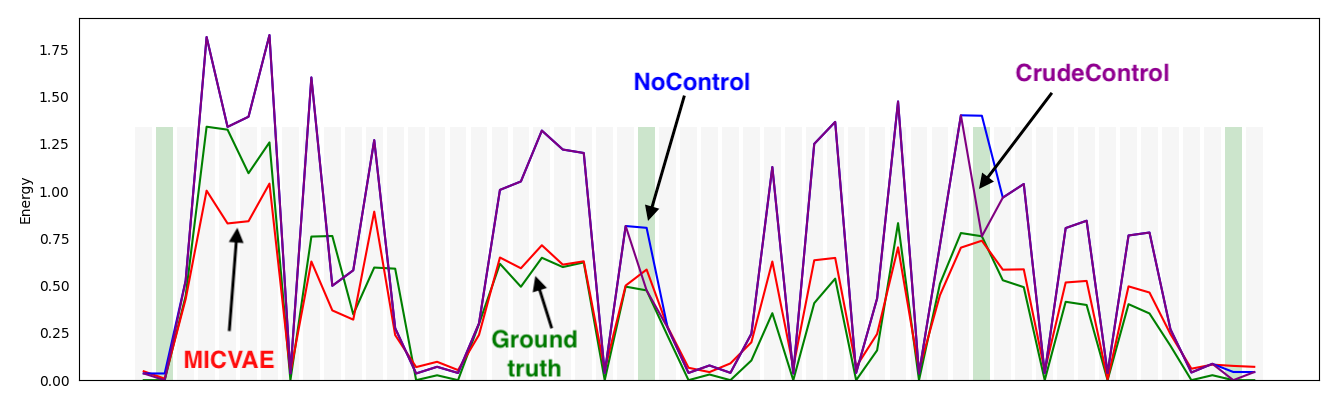
\includegraphics[width=\columnwidth]{figures/demo_a09_08q_004_energy.png}}
    \vskip -0.1in
    \caption{Our model produces plausible prosody, whereas Crude Control produces inconsistent prosody. The control points are shown with green vertical bars.} % \com{Show visually the missing PAFs.}
    \label{fig:demo}
    \vskip -5pt
\end{figure}

\begin{figure}[t]
    \centerline{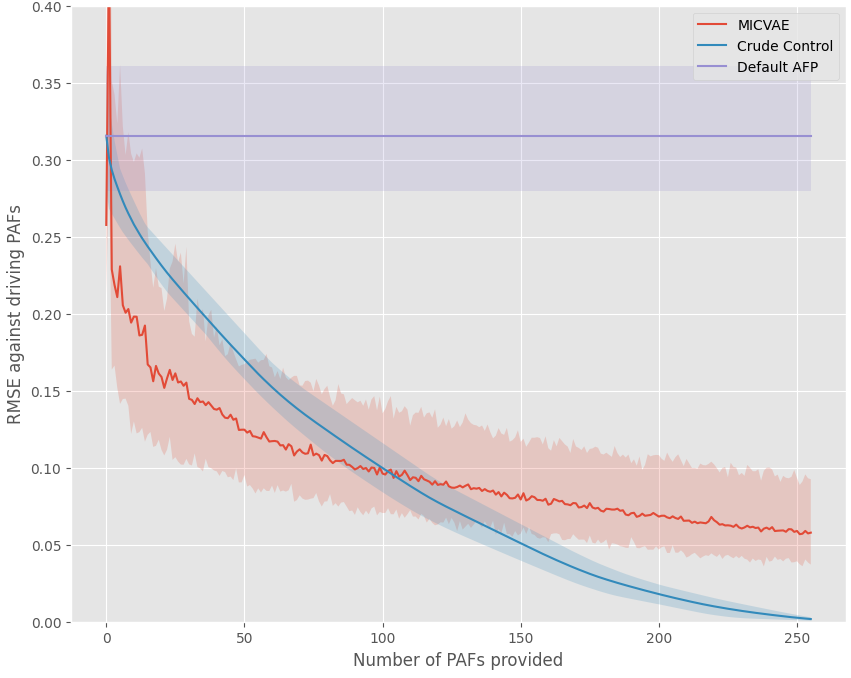
\includegraphics[width=\columnwidth]{figures/efficiency.pdf}}
    \vskip -0.15in
    \caption{Our model controls prosody efficiently. Its generated PAFs are closer to the ground-truth rendition than  is the manually modified output of the AFP, called \sc{CrudeControl}.}
    \label{fig:iterative}
    \vskip -0.2in
\end{figure}

\begin{figure}[t]
    \begin{center}
        \centerline{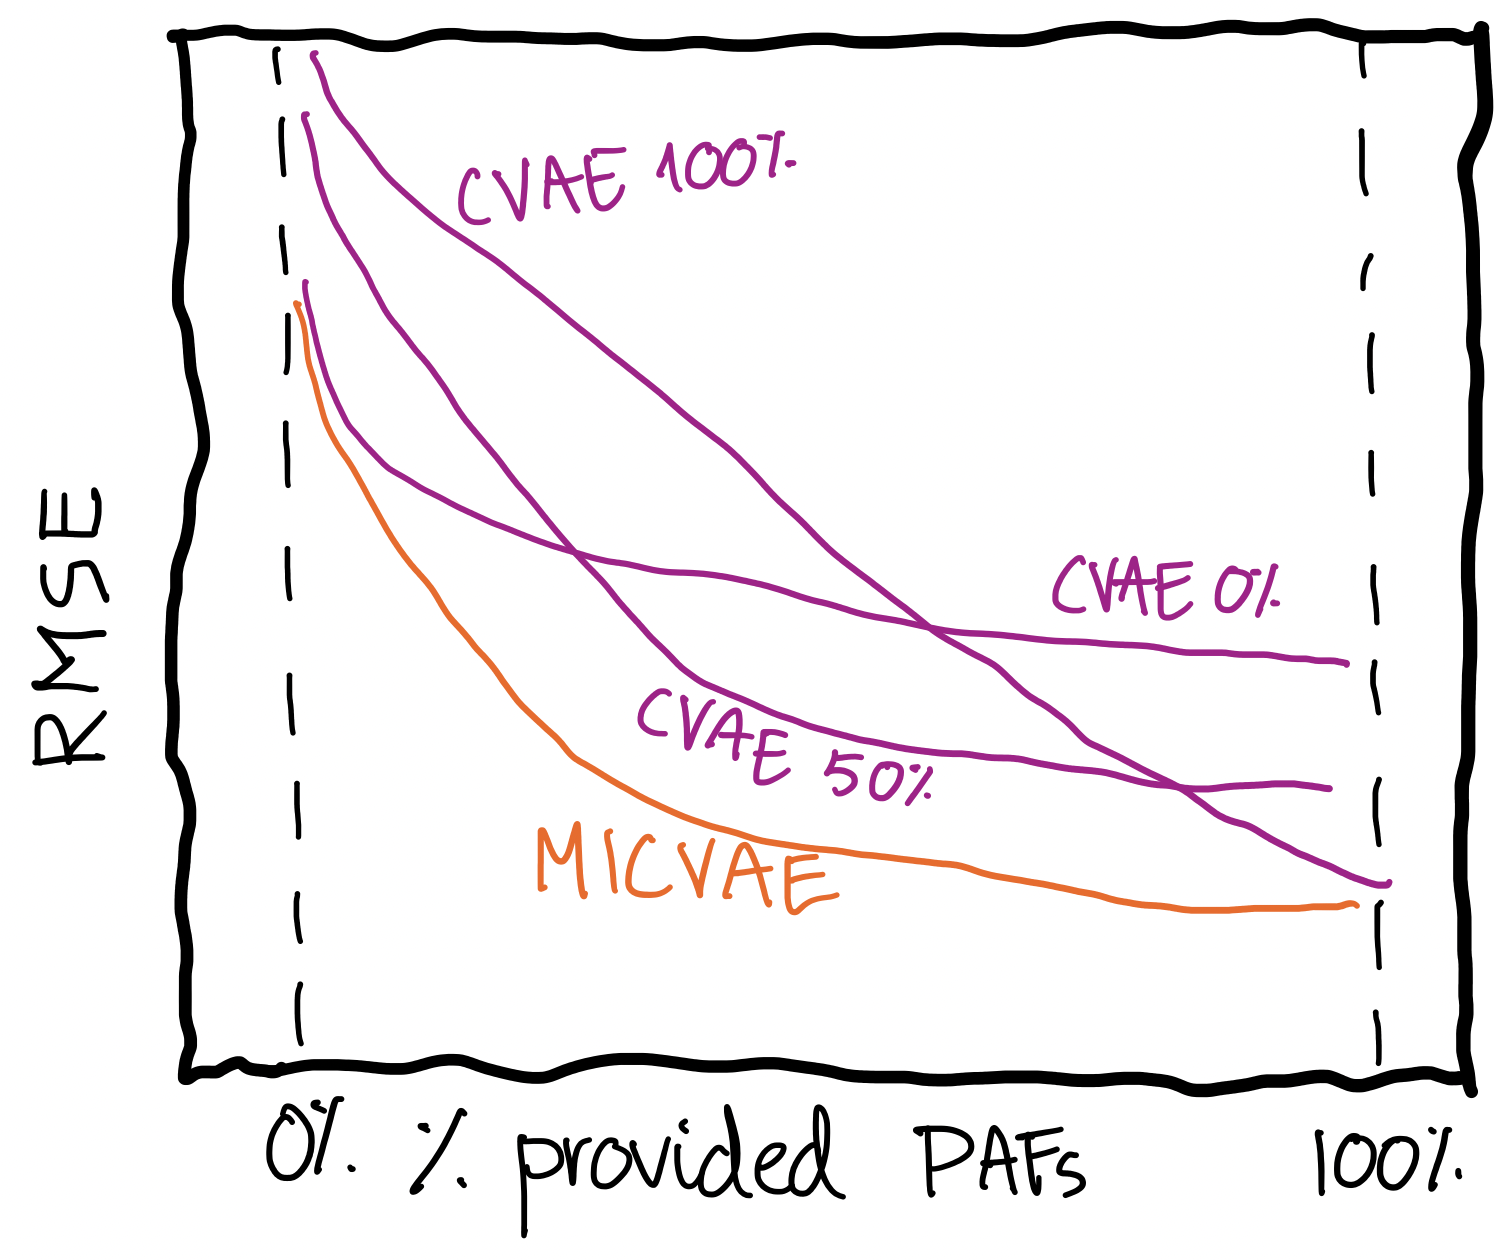
\includegraphics[width=0.9\columnwidth]{figures/robustness.pdf}}
        \vskip -0.15in
        \caption{Our model is robust to changes in the missingness pattern, whereas Masked CVAE only performs well when tested on the same missingness pattern as the one on which it was trained.}\label{fig:robustness}
    \end{center}
    \vskip -0.3in
\end{figure}

\begin{figure}
    \begin{center}
    \centerline{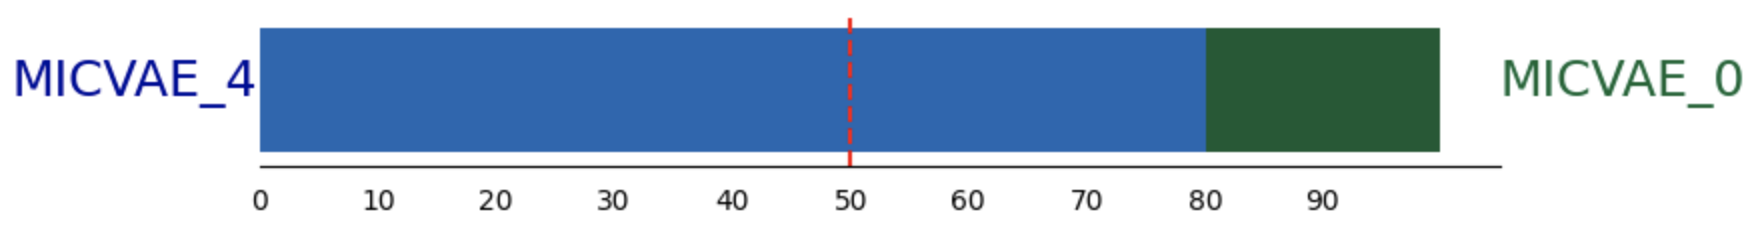
\includegraphics[width=\columnwidth]{figures/faithfulness.png}}
    \vskip -0.15in
    \caption{4 control points are enough to bring our model's output significantly closer to the reference utterance. These are ratings in an A/B/R test where the question is ``Which of these is closer to the reference ground-truth control audio?''.}
    \label{fig:faithfulness}
    \end{center}
    \vskip -0.3in
\end{figure}

Figure~\ref{fig:iterative} reveals that MICVAE significantly outperforms the \textsc{CrudeControl} method, achieving lower RMSEs across a realistic range of missingness (between 4 and 70 PAFs). Our model (MICVAE) produces prosody closer to the ground-truth than the prosody resulting from manually setting the output PAFs to default values, meaning MICVAE uses the learned structure of prosody data to fill in the gaps between the control points. The fact that Crude Control performs better than MICVAE is to be expected when the missingness rate approaches 0, because we are manually switching all PAFs to the values extracted from the ground-truth utterance.

Figure~\ref{fig:faithfulness} reveals that MICVAE with 4 input PAFs is significantly perceived as closer to the reference audio compared to the version without any input PAFs. This not only confirms the model's faithfulness to user intentions but also underscores its efficiency, as it achieves these results with a minimum number of input PAFs.

As illustrated in Figure~\ref{fig:robustness}, MICVAE outperforms all versions of Masked CVAE, even with the same model capacity. The results indicate that Masked CVAEs fail to adapt to varying missingness patterns effectively, emphasizing the robustness of MICVAE. Note that our evaluation results generalise to other generative models than CVAE.\@ We compare different conditioning mechanisms (multiple-instance vs masking) rather than different generator architectures.

% \subsection{Limitations}

% We acknowledge that our work does not investigate all plausible strategies for selecting control points. We explored two strategies: randomly selecting a certain number of PAFs or using iterative refinement (sequentially providing all the PAFs in descending order of reconstruction error). However, other strategies exist, including: 1) Providing PAFs for an entire word. 2) Providing a few PAFs at the beginning and the end of a sentence. 3) Providing only F0 values. A detailed user study would evaluate the utility of our control framework in a range of practical settings.

% Nevertheless, we believe that our quantitative evaluation already demonstrates the effectiveness of our model as a proof of concept. Our work presents a novel problem (efficiency and robustness) and approach (partial inputs) in order to initiate discussion and collaboration within the community. Future research can expand our work by conducting user studies of how humans choose to manipulate PAFs in practice.

% \subsection{Conclusion}

% In this study, we address the challenges of controlling generative models by introducing a new partial-input control framework. We establish three key attributes for a successful generative model: efficiency, robustness, and faithfulness. Our model, derived from the Masked CVAE, empirically exhibits these traits. To enable reproducible testing, we use simulated human-in-the-loop (HitL) control with natural prosodic features extracted from a dataset of repeated utterances. Our work serves as a foundation for future studies on human-in-the-loop control in generative models.

% \crit{A human could mimic the desired prosody within an audio sample. The reviewer's suggestion is insightful, and this technique can already be implemented within our sparse control framework. By speaking the sentence, extracting the PAFs, normalizing them and providing them as control points to MICVAE, we can already condition on audio samples. }

\section{Conclusion} 

\draft{This chapter studies why imputation models trained with 0.5 Bernoulli missingness often fail to generalise to novel patterns of missingness. Our claim is that, when limited network capacity is available, the maximum likelihood solution is not very robust.}

This chapter presents a novel approach to Missing Data Imputation (MDI) using the latent-group model. By using Conditional Variational Autoencoders (CVAEs) and positional embeddings, the method can transform structured data, like time-series, into exchangeable groups. This innovation allows the framework of MDI to tackle complex real-world problems, such as controlling the prosody in Text-To-Speech (TTS) synthesis models, offering efficient and precise human control. The model's efficacy was validated through an iterative refinement procedure and demonstrated robustness to varying patterns of data sparsity. This work contributes significantly to the broader framework of MDI, offering a method for high-dimensional generative model control.

%% WAREHOUSE

% \section{Generalisation of imputation to unseen (non-ignorable) missingness patterns}

% So what is the difference between the model that I am proposing and the way they do it with neural processes? I want to say that my approach is more robust to different patterns of missingness than neural processes. The setup is similar: we have complete data at training time and incomplete data at testing time. The missingness follows an unknown pattern that can be roughly guessed. In my case, I can guess a few patterns, but not all of them.

% Let's back up. What is the problem with imputation on non-ignorable missingness? Many works show that if you try to maximum-likelihood-estimate a parameter based on only complete data from a set of data with non-ignorable missingness, then your estimate will be biased \parencite{rubinInferenceMissingData1976}. In order to get a good estimate of this parameter, we need to model the joint distribution of the data and the missingness \parencite{littleStatisticalAnalysisMissing2002}. We can get provably unbiased estimates of the generative parameters under some (relatively weak) assumptions of the generative model and the missingness mechanism \parencite{maIdentifiableGenerativeModels2021}.

% But this is all for situations where we don't have complete data in the training but instead have a representative sample of the missingness pattern. However, our case comprises something quite different. We have complete data in the training set (but no example of missingness), but we have MNAR missingness at test-time.

% The risk here is no longer that the generative model does not learn the correct distribution. Technically, you can train any latent-variable generative model on the training data, and then, at test-time, use Expectation Maximisation to infer the latent variable corresponding to the partial observations. This procedure would produce an unbiased imputation.

% However, this is too inefficient. In practice, we would use a recognition model to amortise the cost of inferring the latent variable. But the problem is that the parameter of the latent recognition model might be biased. So how can we ensure that the latent recognition model is unbiased?

% There are 2 possible ways:

% \begin{enumerate}
%     \item Come up with a list of sufficient assumptions (that are also quite realistic) for the identifiability of the recognition model.
%     \item Design a model that is more robust to different patterns of missingness, possibly using causal inference.
% \end{enumerate}


% \crit{There are actually 2 chapters here. One is a chapter on the solution for controlling prosody by training with different missingness patterns as a regulariser. Another is a more abstract chapter about what is needed to make amortised function approximation from partial inputs identifiable.}

% Proof of identifiability

% How to call this task? Recovering a conditional distribution from the joint? Not necessarily. Function approximation, but 

% \section{Identifiability of imputation for data missing-not-at-random}

% Missing-not-at-random data is not ignorable when training a regressor with maximum likelihood estimation \parencite{ibrahimMissingDataMethods2009}.

% Some missingness cases are recoverable, depending on the form of the graph \parencite{mohanGraphicalModelsInference2013}.

% \paragraph{Baseline for ignorable missingness.} HI-VAE is the standard VAE-based model for imputing missing data \parencite{nazabalHandlingIncompleteHeterogeneous2020}. They don't assume exchangeability across the dimensions of the data, and they assume a fixed number of dimensions. They do assume that the joint distribution of the dimensions factorises with respect to the latent variable. They maximise likelihood on the observed data and treat the missing data as a latent variable. They don't model the missingness, so they are vulnerable to non-ignorable missingness.

% \paragraph{Identifiable imputation model for non-ignorable missingness.} You can learn an identifiable generative model for MNAR, using the VAE framework, if you make some assumptions first \parencite{maIdentifiableGenerativeModels2021}. They don't assume that you have access to complete cases, but they assume that every feature is observed at least once. They evaluate the model on recommender system (MAR), education responses (MNAR), and a synthetic MNAR dataset. Self-masking means that the value is only masked dependent on the value itself. Their claimed main limitation is the need for auxiliary variables which in practice may not always be available.

% There are 3 assumptions that they make. 1) The true data-generating process is a latent-group model (exchangeable groups) where the masking variable for each element of the group is the causal result of the latent and the corresponding observation, and there is a separate generative parameter for each instance (observation, mask) in the group. 2) There exists a partition of the group in which the joint distribution of each sub-group is identifiable. 3) There exists a cover of the set of elements in the group where the probability of observing the cover is greater than zero.

% Let's look at their implementation of the model, GINA. First of all, they use the encoder for inference, which is wrong, because they assume that the encoder is the same as the prior.

% Let's check out this dissertation and contact the author \parencite{maAdvancesBayesianMachine2022}.

% \paragraph{Identifiable imputation for partially-ignorable missingness} Another paper shows how to perform identifiable imputation for MNAR in a pattern-set mixture model \parencite{ghalebikesabiDeepGenerativeMissingness2021}. Their generative model factorises like this:

% \begin{equation*}
%     \mathbb{P}_\theta (\mathbf{x}^o, \mathbf{x}^u, \mathbf{m}, \mathbf{r}, \mathbf{z}) = \mathbb{P}_\theta (\mathbf{m} | \mathbf{x}, \mathbf{r}) ~ \mathbb{P}_\theta (\mathbf{z} | \mathbf{r}) ~ \mathbb{P}_\theta (\mathbf{r}) \prod_{d} \mathbb{P}_\theta (x^o_d | \mathbf{r}, \mathbf{z}) ~ \mathbb{P}_\theta (x^u_d | \mathbf{r}, \mathbf{z})
% \end{equation*}

% They make the questionable assumption that $\mathbb{P}_\theta (\mathbf{m} | \mathbf{x}, \mathbf{r}) = \mathbb{P}_\theta (\mathbf{m} | \mathbf{z}, \mathbf{r})$. Maybe this is not that questionable.

% \paragraph{Different types of factorisations.} Pattern-set mixture models combine selection and pattern mixture models \parencite{littleStatisticalAnalysisMissing2002}. The random variable $\mathbf{r}$ indicates which pattern of missingness we are talking about.

% \begin{equation*}
%     \mathbb{P}_{\theta, \phi} (\mathbf{x}, \mathbf{m}, \mathbf{r}) = \mathbb{P}_{\theta} (\mathbf{x} | \mathbf{r}) ~ \mathbb{P}_{\phi} (\mathbf{m} | \mathbf{x}, \mathbf{r}) ~ \mathbb{P} (\mathbf{r}) = \mathbb{P} (\mathbf{r}) \sum_{d=1}^D \mathbb{P}_{\theta} (x_d | \mathbf{r}) ~ \mathbb{P}_{\phi} (m_d | \mathbf{x}, \mathbf{r})
% \end{equation*}

% \paragraph{Different types of MNAR.} It turns out that there are different types of data missing-not-at-random. The most obvious kind is called self-censorship, where the missingness depends only on the missing value itself. For example, users might only provide ratings to items they love or hate, but not to items that are neutral.

% Another situation of missingness is the so-called shared parameter model. A shared-parameter model is a certain kind of MNAR that assumes that there exists some structure-level latent variable that, when conditioned, makes the observations independent of the mask \parencite{wuEstimationComparisonChanges1988}. This assumption has been proven to produce more robust models than the MCAR or MAR assumption.

% \begin{equation*}
%     \mathbb{P}_{\theta, \phi} (\mathbf{x}, \mathbf{m}) = \int \mathbb{P}_{\theta} (\mathbf{x} | \mathbf{z}) ~ \mathbb{P}_{\phi} (\mathbf{m} | \mathbf{z}) ~ \mathbb{P} (\mathbf{z}) ~ d\mathbf{z}
% \end{equation*}

% \paragraph{What is specific about our problem statement?} Our problem statement is slightly different from the way most people frame it. We assume that we have complete data at the start, and we want to simulate missingness.

%%%%%%%%%%%%%%%%%%%%%%%%%%%%%%%%%%%%%%%%%%%%%%%%%%%%%%%%%%%%%%%%%%%%%%%%%%%%%%%%
%% References:
%%
% If you include some work not referenced in the main text (e.g. using \nocite{}), consider changing "References" to "Bibliography".
%

% \renewcommand to change default "Bibliography" to "References"
% \renewcommand{\bibname}{References}
\cleardoublepage
\phantomsection
\addcontentsline{toc}{chapter}{References}
% \bibliographystyle{plainnat}
\printbibliography

%%%%%%%%%%%%%%%%%%%%%%%%%%%%%%%%%%%%%%%%%%%%%%%%%%%%%%%%%%%%%%%%%%%%%%%%%%%%%%%%
%% Appendix:
%%

%\appendix

%\chapter{Extra Information}

\end{document}

